

\documentclass[runningheads]{llncs}
%
\usepackage[T1]{fontenc}
% T1 fonts will be used to generate the final print and online PDFs,
% so please use T1 fonts in your manuscript whenever possible.
% Other font encondings may result in incorrect characters.
%
\usepackage{graphicx}
% Used for displaying a sample figure. If possible, figure files should
% be included in EPS format.
%
% If you use the hyperref package, please uncomment the following two lines
% to display URLs in blue roman font according to Springer's eBook style:
%\usepackage{color}
%\renewcommand\UrlFont{\color{blue}\rmfamily}
%\urlstyle{rm}
\usepackage{stfloats}
\usepackage{threeparttable}
\usepackage[table,xcdraw]{xcolor}
\usepackage{hyperref}
\usepackage{multirow}
\usepackage{makecell}
\usepackage{subcaption}
\usepackage{url}
% \usepackage{cite}
\usepackage{algorithmic}
\usepackage{graphicx}
\usepackage{textcomp}
\usepackage{lineno,hyperref}


\usepackage{ragged2e}
\usepackage{graphicx}
\usepackage{textcomp}

\usepackage{footnote}
\usepackage{tcolorbox}

\usepackage[misc]{ifsym}
\usepackage[justification=centering]{caption} 


\usepackage{epsfig,endnotes,amsfonts,bm,tikz,pgfplots}
\usepackage{indentfirst}
% \usepackage[noend]{algpseudocode}
\usetikzlibrary{intersections}
\usetikzlibrary{calc}


\usepackage{framed}
% \usepackage[normalem]{ulem}
% \usepackage{authblk}
\usepackage{enumerate}
% \usepackage[colorlinks]{hyperref}
% \usepackage[pdfstartview=FitH,
%             bookmarksnumbered=true,
%             bookmarksopen=true,
%             colorlinks,
%             pdfborder=001,   %注释掉此项则交叉引用为彩色边框
%             linkcolor=black,
%             anchorcolor=black,
%             urlcolor=black,
%             citecolor=black]{hyperref}
\usepackage[
	lambda,
	advantage,
	operators,
	sets,
	adversary,
	landau,
	probability,
	notions,
% 	logic,
	ff,
	mm,
	primitives,
	events,
	complexity,
	asymptotics,
	keys
	]{cryptocode}
\createprocedurecommand{functionality}{}{\textbf{Functionality~}}{mode=text}
\usepackage{tcolorbox}

\newtheorem{myDef}{Definition} 

\newtheorem{myCor}{Corollary}
\newtheorem{myClaim}{Claim}

\newtheorem{myAx}{Axiom} 


\usepackage{listings}


\usepackage{tikz}
\usetikzlibrary{arrows.meta, positioning, shapes.geometric, backgrounds, fit, calc,shapes.misc}
\definecolor{IEEEblue}{RGB}{0,102,204}



\lstdefinelanguage{Solidity}{
  keywords=[1]{function, mapping, if, else, for, while, return, address, uint, uint256, int, int256, bool, string, bytes, public, private, external, internal, pure, view, payable, new, delete, require, revert, assert, emit, event, modifier, constructor, fallback, receive, using, library, enum, constant, immutable, override, virtual, interface, assembly, uint32},
  keywordstyle=[1]\color{blue},
  keywords=[2]{self, true, false},
  keywordstyle=[2]\color{purple},
  keywords=[3]{TokensReceived, TokensFrozen, TokensSwapped, ComplaintFired, SessionStateUpdated, UserNotified, OrderCreated, SessionCreated, Incentivized, Penalized},
  keywordstyle=[3]\color{purple},
  keywords=[4]{pragma, solidity},
  keywordstyle=[4]\color{cyan},
  keywords=[5]{struct, contract},
  keywordstyle=[5]\color{blue},
  keywords=[6]{G1Point, G2Point, Order, Session, SessionState},
  keywordstyle=[6]\color{orange},
  % identifierstyle=\color{black},
  sensitive=false,
  comment=[l]{//},
  morecomment=[s]{/*}{*/},
  commentstyle=\color{gray}\ttfamily,
  stringstyle=\color{green}\ttfamily,
  morestring=[b]",
  morestring=[b]'
}

\lstset{
  language=Solidity,
  extendedchars=true,
  basicstyle=\ttfamily\small,
  showstringspaces=false,
  showspaces=false,
  numbers=left,
  numberstyle=\tiny,
  numbersep=5pt,
  tabsize=4,
  breaklines=true,
  showtabs=false,
  captionpos=b
}



% \newtheorem{proof}{\mathit{proof}}
\pagestyle{plain} 

\newcommand{\dex}{\mathcal{F}_{\textit{DEX}}}
\newcommand{\swapid}{\mathsf{id}}
\newcommand{\success}{\mathsf{success}}
\newcommand{\failure}{\mathsf{failure}}




\newcommand{\shamirShare}{\mathsf{Share}}
\newcommand{\shamirRecon}{\mathsf{Recon}}

\newcommand{\shamirGShare}{\mathsf{GrpShare}}
\newcommand{\shamirGRecon}{\mathsf{GrpRecon}}


\newcommand{\lsssshare}{\mathsf{LSSSShare}}
\newcommand{\lsssrecon}{\mathsf{LSSSRecon}}
\newcommand{\glsssshare}{\mathsf{GrpLSSSShare}}
\newcommand{\glsssrecon}{\mathsf{GrpLSSSRecon}}


\newcommand{\gssshare}{\mathsf{GSSShare}}
\newcommand{\gssrecon}{\mathsf{GSSRecon}}
\newcommand{\gssreconVrf}{\mathsf{GSSReconWithVrf}}
\newcommand{\ggssshare}{\mathsf{GrpGSSShare}}
\newcommand{\ggssrecon}{\mathsf{GrpGSSRecon}}

\newcommand{\pvgssSetup}{\mathsf{PVGSSSetup}}
\newcommand{\pvgssShare}{\mathsf{PVGSSShare}}
\newcommand{\pvgssVerify}{\mathsf{PVGSSVerify}}
\newcommand{\pvgssPreRecon}{\mathsf{PVGSSPreRecon}}
\newcommand{\pvgssKeyVrf}{\mathsf{PVGSSKeyVrf}}
\newcommand{\pvgssRecon}{\mathsf{PVGSSRecon}}
\newcommand{\pvgssKeyEnc}{\mathsf{PVGSSKeyEnc}}
\newcommand{\pvgssEnKeyVrf}{\mathsf{PVGSSKeyVrf}}
\newcommand{\pvgssGet}{\mathsf{PVGSSGetKey}}



\newcommand{\calZ}{\mathcal{Z}}
\newcommand{\calC}{\mathcal{C}}
\newcommand{\calF}{\mathcal{F}}
\newcommand{\gp}{\mathsf{GP}}
\newcommand{\proofs}{\mathsf{prf}}
\newcommand{\msgset}{\mathcal{M}}

\newcommand{\advind}{\adv_{\textit{IND}}}
\newcommand{\advddh}{\adv_{\textit{DDH}}}


\usepackage{pifont}       % \ding{xx}
\usepackage{bbding}       % \Checkmark,\XSolid,... (需要和pifont宏包共同使用)
\usepackage{fontawesome}  % \faCheck,\faTimes
\newcommand{\cmark}{\ding{51}}%
\newcommand{\xmark}{\ding{55}}%

% \newcommand{\sk}{\textsf{SK}}
% \newcommand{\PK}{\textsf{PK}}

\newcommand{\true}{\textsf{true}}
\newcommand{\false}{\textsf{false}}



% \renewcommand{\arraystretch}{1.22}
\usepackage{amsmath,amssymb,amsfonts}
\usepackage{algorithmic}
\usepackage{graphicx}
\usepackage{textcomp}
\usepackage{xcolor}
\newtcolorbox{functionality2}[2][]{
    colback = white,
    fonttitle = \sffamily\bfseries,
    colbacktitle = white,
    coltitle = black,
    % attach boxed title to top left = {xshift=12pt, yshift=-\tcboxedtitleheight/2},
    boxrule = 0.8 pt,
    % top = \tcboxedtitleheight/2,
    % breakable,
    title=Ideal Functionality\ #2,#1}

\newtcolorbox{functionality3}[2][]{
    colback = white,
    fonttitle = \sffamily\bfseries,
    colbacktitle = white,
    coltitle = black,
    % attach boxed title to top left = {xshift=12pt, yshift=-\tcboxedtitleheight/2},
    boxrule = 0.8 pt,
    % top = \tcboxedtitleheight/2,
    % breakable,
    title=Real Protocol\ #2,#1}    

% to be able to draw some self-contained figs
\usepackage{tikz}
\usepackage{amsmath}




% % to be able to draw some self-contained figs
% \usepackage{tikz}
% \usepackage{amsmath}

% inlined bib file
% \usepackage{filecontents}
%%
%% \BibTeX command to typeset BibTeX logo in the docs
% \AtBeginDocument{%
%   \providecommand\BibTeX{{%
%     Bib\TeX}}}

%% Rights management information.  This information is sent to you
%% when you complete the rights form.  These commands have SAMPLE
%% values in them; it is your responsibility as an author to replace
%% the commands and values with those provided to you when you
%% complete the rights form.
% \setcopyright{acmlicensed}
% \copyrightyear{2025}
% \acmYear{2025}
% \acmDOI{XXXXXXX.XXXXXXX}
% These commands are for a PROCEEDINGS abstract or paper.
% \acmConference[ACM CCS 2025]{Make sure to enter the correct  conference title from your rights confirmation email}{October 13--17, 2025}{Taipei, Taiwan}
% \acmConference[ACM Latex template]{}{2025}{}
%%
%%  Uncomment \acmBooktitle if the title of the proceedings is different
%%  from ``Proceedings of ...''!
%%
%%\acmBooktitle{Woodstock '18: ACM Symposium on Neural Gaze Detection,
%%  June 03--05, 2018, Woodstock, NY}
% \acmISBN{978-1-4503-XXXX-X/18/06}


%%
%% Submission ID.
%% Use this when submitting an article to a sponsored event. You'll
%% receive a unique submission ID from the organizers
%% of the event, and this ID should be used as the parameter to this command.
%%\acmSubmissionID{123-A56-BU3}

%%
%% For managing citations, it is recommended to use bibliography
%% files in BibTeX format.
%%
%% You can then either use BibTeX with the ACM-Reference-Format style,
%% or BibLaTeX with the acmnumeric or acmauthoryear sytles, that include
%% support for advanced citation of software artefact from the
%% biblatex-software package, also separately available on CTAN.
%%
%% Look at the sample-*-biblatex.tex files for templates showcasing
%% the biblatex styles.
%%

%%
%% The majority of ACM publications use numbered citations and
%% references.  The command \citestyle{authoryear} switches to the
%% "author year" style.
%%
%% If you are preparing content for an event
%% sponsored by ACM SIGGRAPH, you must use the "author year" style of
%% citations and references.
%% Uncommenting
%% the next command will enable that style.
%%\citestyle{acmauthoryear}


%%
%% end of the preamble, start of the body of the document source.
\begin{document}

%%
%% The "title" command has an optional parameter,
%% allowing the author to define a "short title" to be used in page headers.
\title{Publicly Verifiable Generalized Secret Sharing Schemes and Their Applications}

\maketitle

\begin{abstract}
% Generalized secret sharing (GSS) enables flexible access control in distributed systems by allowing secrets to be shared across arbitrary monotone access structures.
% However, its adoption in transparent and trustless environments is hindered due to the reliance on trusted participants and secure communication channels.
% This reliance restricts GSS's ability to provide flexible control in the presence of adversaries.
% In this paper, we propose publicly verifiable generalized secret sharing (PVGSS), a scheme that allows to distribute a secret using generalized access structures while enabling non-interactive public verifiability of participant honesty.
% PVGSS scheme offers significant potential to advance the fields of blockchain and applied cryptography, such as attribute-based cryptosystem and on-chain secret escrow.
% Intuitively, we first build two GSS schemes by leveraging recursive Shamir secret sharing and linear secret sharing scheme.
% Then, we encrypt GSS shares and generate the corresponding non-interactive zero-knowledge proofs. Furthermore, we innovatively apply the GSS reconstruction algorithm to show all encrypted shares bind to the dealer's secret, with only \( O(|\mathbb{A}|) \) verification complexity, where \( |\mathbb{A}| \) is the number of leaf nodes in the access structure \( \mathbb{A} \).
% To exemplify the practical applicability, we implement a decentralized exchange (DEX) protocol, where fairness and accountable arbitration are considered.
% Our benchmarks on the BN128 curve demonstrate the computational efficiency of PVGSS schemes, while Ethereum gas cost analysis confirms the viability of the DEX implementation.
Generalized secret sharing (GSS) enables flexible access control in distributed systems by allowing secrets to be shared across arbitrary monotone access structures. However, its adoption in transparent and trustless environments is hindered due to the reliance on trusted participants and secure communication channels. This reliance restricts GSS's ability to provide flexible control in the presence of adversaries. In this paper, we propose publicly verifiable generalized secret sharing (PVGSS), a scheme that allows to distribute a secret using generalized access structures while enabling non-interactive public verifiability of participant honesty. PVGSS scheme offers significant potential to advance the fields of blockchain and applied cryptography, such as attribute-based cryptosystem and on-chain secret escrow. Intuitively, we first build two GSS schemes by leveraging recursive Shamir secret sharing and linear secret sharing scheme. Then, we encrypt GSS shares and generate the corresponding non-interactive zero-knowledge proofs. Furthermore, we innovatively apply GSS testing algorithm to show all encrypted shares bind to the dealer's secret, with only $O(|\mathbb{A}|)$ verification complexity, where $|\mathbb{A}|$ is the number of leaf nodes in the access structure $\mathbb{A}$. To exemplify the practical applicability, we implement a decentralized exchange (DEX) protocol, where fairness and accountable arbitration are considered. Our benchmarks on the BN128 curve demonstrate the computational efficiency of PVGSS schemes, while Ethereum gas cost analysis confirms the viability of the DEX implementation.

\keywords{Access structure, Public verifiability, PVGSS, GSS Testing, Decentralized exchange}
\end{abstract}




% \section*{Track Justification Statement}
% This work introduces a novel cryptographic primitive, PVGSS, making the Applied Cryptography track the most appropriate fit. It also presents a decentralized exchange on Ethereum, positioning the Blockchain and Distributed Systems track as a secondary fit.





\section{Introduction}
\label{sec:introduction}

% Secret sharing (SS)~\cite{Shamir79SS}, followed by threshold cryptography~\cite{sahai2005fuzzy} and  distributed key generation~\cite{Das2022DKG}, forms the foundational basis of quorum-based trust. Initially, this trust is instantiated through a fixed threshold of participants, and later generalized~\cite{Ito1987GSS,benaloh1990generalized,Beimel2025GSS} via access structures that codify the trusted subsets of parties.
% The concept of verifiable secret sharing (VSS)~\cite{Feldman1987VSS,Bagherpour2022VPSS,Alon1995VSS} extends this foundation to ensure that the sharing process is correctly executed. This guarantees that any qualified quorum can successfully reconstruct the secret in the future, assuming the initial sharing was valid.
% Verifiability typically incurs additional coordination and interaction during the sharing phase. In contrast, public verifiable secret sharing (PVSS)~\cite{Stadler1996PVSS,Cascudo2017PVSS,cascudo2024publicly} allows any party—without collaboration—to independently verify the correctness of the sharing using publicly available information.

% In contemporary decentralized architectures, such as blockchain-based Web 3.0 systems, it is increasingly critical to ensure fine-grained access control while enabling autonomous public verification by individual agents to strengthen accountability~\cite{Cao2025Web3}. On the one hand, one-to-many data sharing with flexible access policies allows secret reconstruction by diverse and dynamic subsets of participants. On the other hand, detecting faulty behaviors throughout the entire data lifecycle is essential for safeguarding data sovereignty and enforcing privilege boundaries. Against this backdrop, the design of publicly verifiable generalized secret sharing (PVGSS) schemes emerges as a particularly compelling direction.


% A PVGSS scheme should simultaneously support two key properties: generalized access structures (GAS), which supports flexible quorum structures and generalized access policies; and public verifiability, which enables both the dealer and the shareholders to be held accountable in a non-interactive manner.
% In comparison to existing SS-based cryptographic schemes, several limitations emerge. (i) VSS and PVSS are typically tailored to threshold structures and do not natively support generalized access policies. (ii) Linear secret sharing schemes (LSSS)~\cite{Karchmer1993LSSS,Beimel2011LSSS,Beimel2025GSS}, along with VSS, generalized secret sharing (GSS)~\cite{Ito1987GSS,benaloh1990generalized,Beimel2025GSS}, and verifiable generalized secret sharing (VGSS)~\cite{Herranz2003VGSS}, generally assume the existence of private channels for share distribution and lack mechanisms for public verifiability. (iii) Ciphertext-policy attribute-based encryption (CPABE)~\cite{Bethencourt2007CPABE,Lewko2011DABE}, while supporting expressive access control, does not incorporate built-in guarantees for the honest behavior of encryptors or authorities.
% % Table~\ref{table:ss_comparison} summarizes a comparison of the functional capabilities by different cryptographic primitives.


% A PVGSS construction is not simply a direct composition of VSS or PVSS instances, which makes its implementation particularly challenging. The central challenge lies in designing non-interactive zero-knowledge (NIZK) proofs that convincingly demonstrate the encrypted shares \(\{C_i\}\) are correctly bound to the underlying secret \(s\).
% In this paper, we aim to implement PVGSS schemes built upon a GSS framework, which can be instantiated using either recursive secret sharing or LSSS.
% We first encrypt each GSS share $s_i$ as $C_i=\pk_i^{s_i}$, where $\pk_i$ is the public key of shareholder $P_i$. 
% Then, we employ the Sigma protocol~\cite{damgaard2002sigma} and the Fiat-Shamir heuristic~\cite{fiat1986prove} to generate NIZK proofs for each share.
% % \footnote{Similar to the Albatross PVSS scheme~\cite{cascudo2020albatross}, we also employ the Sigma protocol and the Fiat-Shamir heuristic to obtain NIZK proofs. However, since PVGSS is not simply a combination of multiple PVSS instances, it diverges significantly from Albatross—as detailed in Section~\ref{sec:comparison_with_albatross}.} 
% Importantly, we leverage partial data—specifically, the response values \(\{\hat{s}_i\}\) from the Sigma protocol—to construct proofs that establish the binding relationship between the encrypted shares and the underlying secret, utilizing the \(\gssrecon\) algorithm (cf. Definition~\ref{def:GSS}).
% Our solution emphasizes the careful integration of GSS to address the binding relationship between shares and the secret, thereby enabling the construction of PVGSS schemes.

Secret sharing (SS)~\cite{Shamir79SS} and its subsequent extensions, including threshold cryptography~\cite{sahai2005fuzzy} and distributed key generation (DKG)~\cite{Das2022DKG}, constitute a foundational primitive for quorum-based trust in distributed systems. To ensure correctness of the sharing process, verifiable secret sharing (VSS)~\cite{Feldman1987VSS,Bagherpour2022VPSS,Alon1995VSS} and publicly verifiable secret sharing (PVSS)~\cite{Stadler1996PVSS,Cascudo2017PVSS,cascudo2024publicly} were introduced, enabling participants or even external observers to verify that a dealer has distributed consistent shares.

% Despite these advances, existing secret sharing paradigms remain insufficient for modern decentralized systems. On the one hand, emerging applications—such as blockchain, Web 3.0~\cite{Cao2025Web3}, and decentralized finance—require \emph{fine-grained access control} that goes beyond simple threshold policies. On the other hand, the trustless nature of these systems necessitates \emph{non-interactive public accountability}, whereby any observer can independently verify the correctness of secret distribution without relying on trusted channels or coordinated interaction. Reconciling these two requirements remains an open challenge.
Despite substantial progress, existing secret sharing paradigms remain ill-suited for modern decentralized systems. Emerging applications—such as blockchain, Web~3.0~\cite{Cao2025Web3}, and decentralized finance—demand expressive access control beyond simple threshold policies, enabling hierarchical, weighted, or composite authorization. Meanwhile, the trustless nature of these systems requires non-interactive public verifiability, so that any external observer can validate correctness without private channels or trusted coordination. Reconciling expressiveness with public verifiability thus constitutes a fundamental and unresolved challenge, rather than an incremental extension of existing techniques.


Generalized secret sharing (GSS)~\cite{Ito1987GSS,benaloh1990generalized,Beimel2025GSS} addresses the expressiveness gap by supporting arbitrary monotone access structures. However, classical GSS constructions assume private communication channels and do not provide mechanisms for public verifiability. Conversely, PVSS schemes~\cite{Stadler1996PVSS,Cascudo2017PVSS,cascudo2024publicly} achieve public verifiability but are inherently restricted to threshold access structures. Ciphertext-policy attribute-based encryption (CPABE)~\cite{Bethencourt2007CPABE,Lewko2011DABE} supports expressive access policies, yet lacks built-in guarantees that encryptors or authorities behave honestly, rendering accountability external to the primitive. The linear secret sharing scheme (LSSS)~\cite{Karchmer1993LSSS,Beimel2011LSSS,Beimel2025GSS} forms the foundational tool enabling expressive mechanisms in many CPABE schemes.

In this work, we initiate the study of publicly verifiable generalized secret sharing (PVGSS), which simultaneously supports generalized access structures and non‑interactive public verifiability. A PVGSS scheme satisfies two core properties. \emph{Expressiveness} enables secrets to be protected under arbitrary monotone access policies, thereby advancing research on attribute‑based encryption~\cite{Bethencourt2007CPABE,Lewko2011DABE} in trustless environments. \emph{Public verifiability} ensures that both dealers and shareholders can be held non‑interactively accountable by any verifier, making PVGSS particularly well‑suited for blockchain settings, where on‑chain secret management or governance~\cite{Benhamouda2020Secret,Goyal2022Secret,Cerulli2023Secret}, scaling~\cite{Dziembowski2018Channel} and chain interoperability~\cite{Xie2022zkBridge,Park2023Oracle} impose stringent requirements.
% Moreover, real‑world distributed cryptosystems—such as distributed randomness beacon protocols~\cite{Choi2023Beacon}—can leverage PVGSS to facilitate weighted privilege and to improve scalability.
To enhance clarity and emphasize the necessity of PVGSS, we present a comparison with existing SS-based schemes in Table~\ref{table:ss_comparison}.



\newcommand\MyHead[2]{%
  \multicolumn{1}{|c|}{\parbox{#1}{\centering #2}}
}
\renewcommand{\arraystretch}{1.2}
\begin{table}[!h]

% \begin{threeparttable}
\caption{Comparison of SS-related cryptographic primitives}\label{table:ss_comparison}
    \begin{center}    
    \scalebox{1}{\begin{tabular}{ |l|c|c|c|c|c| }
        \hline
        Scheme & \MyHead{2cm}{Accountable dealer (or encryptor)}
         & \MyHead{2.2cm}{Accountable shareholders (or authorities)} &
         \MyHead{1.2cm}{Insecure\\ channel} &
         \MyHead{1.6cm}{Public\\ verifiability} & \MyHead{2.2cm}{Expressiveness}\\
        % \cmidrule(r){1-1}\cmidrule(rl){2-2}\cmidrule(rl){3-3}\cmidrule(rl){4-4}\cmidrule(l){5-5}
        \hline
        SS & \xmark & \xmark & \xmark & \xmark & \xmark\\       
        VSS & \cmark & \xmark & \xmark & \xmark & \xmark\\
        PVSS & \cmark & \cmark & \cmark & \cmark & \xmark\\   
        CPABE & \xmark & \xmark & \cmark & \xmark & \cmark\\
        LSSS& \xmark & \xmark & \xmark & \xmark & \cmark\\
        GSS & \xmark & \xmark & \xmark & \xmark & \cmark\\
        \textbf{PVGSS} & \cmark & \cmark & \cmark & \cmark & \cmark\\
        \hline
    \end{tabular}}
\begin{tabular}{p{12cm}}
    $\bullet$ Accountability indicates whether misbehavior by dealers (or encryptors) and shareholders (or authorities) can be detected.\\
    $\bullet$ Insecure channel denotes that secret shares may be distributed over public channels.\\
    $\bullet$ Public verifiability means that correctness can be checked by any external party.\\
    $\bullet$ Expressiveness indicates native support for arbitrary monotone access structures.\\
\end{tabular}
\end{center}
\end{table}


% Achieving PVGSS is non-trivial: a PVGSS construction cannot be obtained by a naïve composition of PVSS instances, as this would violate correctness under generalized access structures.
Crucially, PVGSS cannot be obtained by naively combining existing PVSS schemes. The core technical challenge of PVGSS is to prove, in a publicly verifiable manner, that a collection of encrypted shares \(\{C_i\}\) is globally consistent with a single underlying secret under an arbitrary access structure. Suppose the access structure is represented as a tree, the secret is associated with the root while encrypted shares are assigned only to the leaf nodes, rendering any straightforward combination of multiple PVSS instances ineffective.
To overcome this challenge, we build PVGSS schemes atop the GSS framework, instantiated using either recursive Shamir secret sharing or linear secret sharing schemes (LSSS). Each GSS share \(s_i\) is encrypted under the public key of shareholder \(P_i\) and is accompanied by non‑interactive zero‑knowledge (NIZK) proofs derived from Sigma protocols~\cite{damgaard2002sigma} via the Fiat–Shamir heuristic~\cite{fiat1986prove}. 
Furthermore, we propose a verification algorithm (i.e., GSS testing) to enable validity checks for all shares over an arbitrary access structure. With this algorithm, we establish a binding relation between all encrypted shares and the dealer’s secret, thereby elegantly resolving the challenge of public verifiability in secret sharing over general access structures. 
% Importantly, the verification complexity remains linear in the number of leaf nodes of the access structure \(\mathbb{A}\), i.e., \(\mathcal{O}(|\mathbb{A}|)\).







\subsection{Applications}
\label{sec:other_applications}
PVGSS introduces a cryptographic primitive that simultaneously supports expressive access control and non-interactive public accountability—two properties that rarely coexist in prior systems. This combination enables new capabilities across several security-critical domains where correctness must be verifiable by untrusted observers and where access policies extend far beyond simple thresholds.
In Section~\ref{sec:dex_on_pvgss}, we will dive deep into a decentralized exchange (DEX) protocol applying PVGSS.


\paragraph{Large-scale beacon protocols.}
Existing PVSS-based distributed randomness beacons~\cite{Choi2023Beacon} protocols are fundamentally constrained by threshold policies, limiting committee flexibility and preventing hierarchical or weighted participation. PVGSS enables publicly verifiable share consistency under arbitrary monotone structures, allowing beacon protocols to incorporate multi-tier committees, heterogeneous trust assumptions, and application-specific quorum rules without sacrificing transparency. This expands the design space for scalable, decentralized randomness generation.
For example, by partitioning $n$ distributed parties into subgroups of size $c$, one can define an access control policy of the form  
$(d \text{ of } (\frac{c}{3} \text{ of } P_1,\ldots,P_c), (\frac{c}{3} \text{ of } P_{c+1}$, $\ldots,P_{2c}), \ldots, (\frac{c}{3} \text{ of } P_{(\frac{n}{c}-1)c+1},\ldots,P_n))$, where the parameter $d$ is introduced to balance unpredictability and liveness of the beacon~\cite{Syta2017Beacon,Schindler2020Beacon}. Under this policy, each party communicates only with a small subgroup of peers, thereby improving scalability.


\paragraph{Attribute-based cryptosystem.} PVGSS can significantly enhance attribute-based cryptosystems~\cite{Bethencourt2007CPABE,Lewko2011DABE} by ensuring trust and transparency in key distribution and access control. By replacing LSSS with a PVGSS, a CPABE scheme can be directly transformed into one that is secure against chosen-ciphertext attacks. Moreover, PVGSS enables CPABE encryptors to outsource encryption to untrusted servers while ensuring public accountability for their behaviors.
    

\paragraph{Blockchain ecosystems.} 
Blockchain environments require protocols that operate over public channels, tolerate adversarial participants, and provide transparent correctness guarantees. PVGSS naturally applies to the scenarios below:

$\bullet$ PVGSS, functioning as a timed commitment~\cite{tyagi2023riggs}, can be effectively used in on-chain \textbf{secret escrow} systems~\cite{Benhamouda2020Secret,Goyal2022Secret,Cerulli2023Secret} to provide fine-grained and verifiable management of witnesses, thereby facilitating practical deployments of e‑voting and auction protocols.

$\bullet$ In blockchain \textbf{bridges}~\cite{Xie2022zkBridge}, PVGSS ensures that the secret values used to lock and release assets are verifiably shared, thereby coordinating data synchronization across multiple validators or blockchains under a single access control policy.

$\bullet$ In \textbf{relay networks}~\cite{Li2022Bridge}, PVGSS enables secure forwarding of state proofs with public verifiability among different groups or committees.

$\bullet$ In payment or state \textbf{channels}~\cite{Dziembowski2018Channel}, PVGSS supports flexible quorum policies for dispute resolution, allowing participants to reconstruct secrets only under authorized conditions.

$\bullet$ Incorporating PVGSS into \textbf{oracle}~\cite{Park2023Oracle} design strengthens functionality by ensuring decentralized, publicly verifiable data feeds and enabling flexible privilege weighting among oracle nodes.

$\bullet$ By designing robust access control structures, KYC/AML (i.e., the compliance measurements of know your customer/ anti money laundering) can be effectively enforced as required by \textbf{stablecoin governance}. For example, an access policy such as  \((3 \text{ of } (Alice,\) \(Bob, (t \text{ of } Reg_1,\cdots, Reg_n)))\) enables a threshold number of regulators to transparently monitor the transaction between exchangers (i.e., Alice and Bob).  



 % \item \textbf{Searchable encrypted database}

\subsection{Contributions}

$\bullet$ We introduce Publicly Verifiable General Secret Sharing (PVGSS)--the first secret sharing framework that simultaneously supports arbitrary monotone access structures and non-interactive public verifiability.
    This resolves a long-standing tension between the expressiveness of general secret sharing (GSS) and the accountability of publicly verifiable schemes.

$\bullet$ We present two PVGSS instantiations: one built atop recursive Shamir secret sharing and the other derived from linear secret sharing schemes (LSSS). 
First, the individual encrypted shares are validated using Sigma‑protocol–based NIZK proofs. Furthermore, we establish a binding relationship between the encrypted shares and the dealer’s secret by means of a proposed GSS testing algorithm, which relies exclusively on existing NIZK proof transcripts as input.  
% The overall verification complexity remains linear in the number of leaf nodes in the access structure.

$\bullet$ Apart from correctness and verifiability, we formalize the security notions of IND1-secrecy and public verifiability for PVGSS, and rigorously prove that our constructions are secure under the standard Decisional Diffie-Hellman (DDH) assumption in the random oracle model.

$\bullet$ To validate the practicality of PVGSS, we design and implement a novel DEX protocol that achieves optimistic fairness, stateless arbitration, and on-chain accountability. Our Ethereum‑compatible prototype executes swaps for less than \$0.55 USD in a 9‑arbitrageur setting in the optimistic case, demonstrating strong real‑world viability.




% \subsection{Paper Organization}

% Section~\ref{sec:introduction} introduces the motivation, application scenarios, and main contributions of PVGSS. Section~\ref{sec:related_works} surveys related work, including threshold-based and generalized secret sharing, as well as publicly verifiable systems, positioning PVGSS within the broader cryptographic landscape.
% Section~\ref{sec:preliminaries} provides necessary preliminaries on access structures, Shamir and LSSS-based secret sharing, and Sigma protocols. Section~\ref{sec:gss} formally defines the Generalized Secret Sharing (GSS) scheme and presents two constructions—Shamir-based and LSSS-based—along with their correctness and secrecy properties.
% Section~\ref{sec:pvgss} introduces the full PVGSS scheme, detailing its syntax, algorithms, and security model. It also formally analyzes the proposed constructions under the DDH assumption. Section~\ref{sec:dex_on_pvgss} demonstrates a practical application of PVGSS in building a decentralized exchange (DEX) that ensures fair token swaps and accountable arbitration.
% Section~\ref{sec:experiments} reports experimental results, including monetary cost on Ethereum blockchain. Section~\ref{sec:conclusion} concludes the paper and outlines future work.   The appendix summarizes the global states using smart contract pseudocode.

\section{Related Works}
\label{sec:related_works}


\subsection{Access Structures in Secret Sharing}

As is well known, traditional SS, VSS, and PVSS  protocols~\cite{Shamir79SS,Feldman1987VSS,Stadler1996PVSS,Cascudo2017PVSS,cascudo2024publicly} are designed around the threshold access structure (TAS). 
Benaloh et al.~\cite{benaloh1990generalized} introduced the concept of generalized secret sharing (GSS) based on recursive threshold secret sharing, where generalized access structure (GAS) is inherently implied. Beyond  TAS- or GAS- based schemes, some other protocols have explored specific types of access control mechanisms. 
% To unify these protocols, we refer to them as multi-level secret sharing schemes.


In particular, Simmons~\cite{Simmons1988SS} points out that real-world applications require more versatile capabilities for secret sharing. 
In weighted secret sharing (WSS)~\cite{beimel2005characterizing,Garg2023MPC}, each participant is assigned a positive weight. Only if the sum of weights of some participants exceeds the predefined threshold value, can the secret be reconstructed. 



In multipartite secret sharing (MSS)~\cite{Chen2021MSS,tassa2009multipartite}, an access structure defined over $n$ participants is partitioned into disjoint $m(\ll n)$ compartments, where participants within the same compartment have equal weights. In MSS, each compartment must achieve a specific internal agreement before contributing to the reconstruction of the secret. 
Tassa et al.~\cite{tassa2009multipartite} point out that any GAS can be regarded as a multipartite access structure with singleton compartments. Hence, reconstructing the secret in MSS scheme depends only on the number of participants from each compartment, rather than their individual identities. In this way, practical applications can focus on $m$ compartments, where TAS is applied, instead of $n$ individuals. However, participants may be designed in different access structures in a single system, resulting in different divisions of disjoint compartments.




 % Farràs, O., Martí-Farré, J. and Padró, C., 2012. Ideal multipartite secret sharing schemes. Journal of cryptology, 25(3), pp.434-463.


Hierarchical secret sharing (HSS)~\cite{tassa2007hierarchical,Chattopadhyay2024SS}, also referred as multilevel secret sharing~\cite{Simmons1988SS,tassa2007hierarchical}, places participants in disjoint levels according to their importance. HSS can be applied in managing staff in big companies, where employees are assigned to different levels with different privileges. 
HSS is categorized into disjunctive and conjunctive types~\cite{Drăgan2016DWSS}. Further, Drăgan et al.~\cite{Drăgan2016DWSS} introduce the distributive weighted threshold secret sharing, where participants at the same level have the same weight, and the threshold values are 1.

Other related works, such as proactive secret sharing~\cite{Bagherpour2022VPSS} and multiple secret sharing~\cite{Lin2018PVMSS}, can be regarded as extensions of SS. Moreover, these concepts can also be incorporated into our GSS and PVGSS schemes.

% graph-based access structure
 

% Though GSS may not "ideal"~\cite{Drăgan2016DWSS,beimel2005characterizing,Chen2021MSS,tassa2009multipartite}, GSS can satisfy the application scenarios where MSS, WSS or HSS apply. 

% \subsection{Public Verifiability}
% Public verifiability is a property that allows any third party to verify the correctness of a computation or data without accessing private information. It is crucial in systems like blockchain~\cite{Scafuro2019PV}, e-voting~\cite{Huber2022Voting}, fair exchange~\cite{Thyagarajan2022Swap,Zhang2024OFE}, and secure MPC~\cite{Baum2020MPC}, where transparency and trust are essential.
% Public verifiability enhances accountability, reduces reliance on trusted parties, and ensures integrity in decentralized environments. 


% Blockchain's momentum over the past decade stems from its ability to ensure transparency, decentralization and smart contracts.
% % It revolutionizes industries by enabling trustless systems~\cite{Zamyatin2019Xclaim}, empowering individuals~\cite{Dunphy2018DID}, and fostering innovation in finance, healthcare, and global collaboration.
% Transactions on the blockchain are considered publicly verifiable, as the operations within these transactions are replicated across distributed nodes.
% To further safeguard privacy of private keys and sensitive information while executing transactions in a transparent environment, various cryptographic tools are widely adopted.

% Merkle tree~\cite{Szydlo2004Merkle} and accumulators~\cite{Kemmoe2024Acc} are often employed to prove membership of specific data in a set publicly. Digital signature schemes~\cite{Schnorr1990Sig,Erwig2021Adaptor} are leveraged to achieve authentication, i.e., enabling public verifiability of identities.
% Verifiable random function (VRF)~\cite{Gilad2017Algorand} is a cryptographic primitive that generates pseudorandom outputs along with a proof, allowing anyone to verify the correctness of the output without revealing the secret key. 
% % Verifiable computation~\cite{Ateniese2007PDP} enables a client to outsource computation to a server (or prover) and efficiently verify the correctness of the result without re-executing the computation. 

% NIZK systems, such as Fiat-Shamir heuristic-based Sigma protocol~\cite{damgaard2002sigma, fiat1986prove} and zkSNARK~\cite{Setty2020ZK}, are often adopted to prove knowledge of plaintext or correctness of operations in a public manner. 
% For instance, the discrete logarithm equality algorithm, based on Sigma protocol, allows a prover to convince any verifier that two group elements share the same exponentiation. 
% Similarly, zkRollup is a scaling solution for blockchains that leverages zkSNARK to bundle multiple transactions into a single proof~\cite{Polygon2023ZK}. By processing transactions off-chain and submitting only a compact zkSNARK proof to the main chain, zkRollups drastically reduce data load and gas costs while ensuring security and privacy. 

% % The construction and broader potential applications of GSS are still being explored and developed. 

\subsection{(Publicly) Verifiable Secret Sharing}
Dealer in the SS scheme may distribute invalid shares to deviate from the protocol. 
To mitigate this problem, VSS~\cite{Feldman1987VSS,Abraham2023VSS} ensures that participants can verify the validity of the shares distributed by the dealer, while PVSS~\cite{Stadler1996PVSS, Cascudo2017PVSS} extends this by allowing any external observer to verify the integrity of the shares. Notably, Galil and Yung~\cite{Galil1987} combine VSS, partition encryption and NIZK proofs to design a more efficient and fully polynomial scheme known as partitioned VSS.


The first VSS scheme, proposed by Feldman~\cite{Feldman1987VSS}, enhances Shamir secret sharing by adding public commitments to ensure share validity. Shareholders verify their shares against these commitments, ensuring the dealer's honesty without revealing the secret. 
Recently, polynomial commitments~\cite{Kate2010VSS, Abraham2023VSS,Zhang2024VSS} are widely adopted to design new VSS schemes. The secret shares of VSS should not be transferred publicly.


Stadler~\cite{Stadler1996PVSS} put forward the first PVSS scheme in 1996. Intuitively, PVSS can be achieved by integrating public key encryption into VSS schemes, allowing secret shares to be delivered and verified on public channels. For example, ElGamal, RSA, and Pailler cryptosystems are utilized in \cite{Stadler1996PVSS, Schoenmakers1999PVSS}, \cite{Fujisaki1998PVSS}, and \cite{Ruiz2005PVSS}, respectively.
Early PVSS schemes require $O(nt)$ verification complexity, where $n$ and $t$ are the amount of shareholders and threshold value, respectively.
In 2017, Cascudo et al.~\cite{Cascudo2017PVSS} introduced SCRAPE PVSS which for the first time achieves $O(n)$ verification complexity. As the core technique, Reed-Solomon code is employed to make all encrypted shares be verified in a linear operation.

Recently, Cascudo et al. successively proposed ALBATROSS~\cite{cascudo2020albatross}, HEPVSS/DHPVSS~\cite{cascudo2022yolo}, and qCLPVSS~\cite{cascudo2024publicly}, which all maintain $O(n)$ verification complexity. ALBATROSS~\cite{cascudo2020albatross} leverages low-degree exponent interpolation to generate NIZK proof, which is essentially acquired from Sigma protocol and Fiat-Shamir heuristic.
HEPVSS\cite{cascudo2022yolo} also uses ElGamal to encrypt the secret share, while DHPVSS\cite{cascudo2022yolo} leverages Shamir secret sharing on group $\GG$ to hide shares.
qCLPVSS~\cite{cascudo2024publicly} enables users to recover the original secret $s\in \ZZ_q$ by leveraging class group, making it applicable in more wider applications, such as distributed key generation~\cite{Das2022DKG,cascudo2024publicly} and MPC~\cite{cascudo2024publicly,cascudo2022yolo} protocols.




\section{Preliminaries}
\label{sec:preliminaries}

In this paper, \( \ZZ_q \) denotes a finite field with prime order \( q \), and \( \GG \) represents a cyclic group of the same order generated by \( g \).
 


\subsection{Generalized Access Structure (GAS)}

\begin{definition}[GAS~\cite{benaloh1990generalized,Lewko2011DABE}]
\label{lab:access_structure}
Let $\mathcal{P}=\{P_1,\cdots,P_n\}$ be a set of parties. A collection $\mathbb{A}\in 2^\mathcal{P}$ is a generalized access structure (GAS, commonly abbreviated as AS in previous research~\cite{benaloh1990generalized,Lewko2011DABE}), if it meets the following two conditions:
\begin{itemize}
\item Non-triviality: if $B\in\mathbb{A}$, then $|B|\neq 0$.
\item Monotonicity: if $B\in \mathbb{A}$, $B  \subseteq  C$, then $C \in\mathbb{A}$.
\end{itemize}
If $B\in \mathbb{A}$, we say $\mathbb{A}$ is satisfied by $B$ or $B$ is an authorized set; Otherwise, $\mathbb{A}$ is not satisfied by $B$ or $B$ is unauthorized.
\end{definition}

% Figure~\ref{fig:boolean_acp} and Figure~\ref{fig:threshold_acp} illustrate examples of two categories of access structure, i.e., $(P_1 \wedge P_2) \vee (P_2 \wedge P_3)$ and $1\ of\ (2\ of$ $(P_1, P_2, P_3), (1\ of$ $\ (P_1, P_4)))$.

\begin{figure}[!h]
    % \centering    
    \begin{minipage}[t]{0.5\textwidth} 
        \centering
        \includegraphics[width=0.8\textwidth]{boolean_acp.eps} 
        \caption{An access structure using boolean formula, where $\{P_{1,1}, P_{2,1}\}$ and $\{P_{2,*}, P_{3,1}\}$ are authorized sets.\label{fig:boolean_acp}} 
    \end{minipage}
% \end{figure}
% \begin{figure}[!h]
    % \hspace{0.05\textwidth}      
    \begin{minipage}[t]{0.5\textwidth} 
        \centering
        \includegraphics[width=0.95\textwidth]{threshold_acp.eps} 
        \caption{An access structure using threshold gate, where $\{P_{3,1}, P_{2,*}\}$ and $\{ P_{1,1}, P_{3,1}, P_{4,1}\}$ are authorized sets.\label{fig:threshold_acp}} 
    \end{minipage}
\end{figure}

For example, $(P_{1,1} \wedge P_{2,1}) \vee (P_{2,2} \wedge P_{3,1})$ and $2\ of\ (2\ of$ $(P_{1,1}, P_{2,1},$ $ P_{3,1}), (1\ of$ $\ (P_{1,2}, P_{4,1})))$ are access structures, as shown by Figure~\ref{fig:boolean_acp} and Figure~\ref{fig:threshold_acp}, where $P_{i,j}$ represents the $j$th authorization granted to party $P_i$ and $*$ is a wildcard. The disjunction ($\vee$) and conjunction ($\wedge$) in a boolean formula based access structure (cf. Figure~\ref{fig:boolean_acp}) is equal to the gate value of 1 and 2 in a threshold-gate based access structure (cf. Figure~\ref{fig:threshold_acp}), respectively. Hence, we only consider threshold-gate based access structure in this paper. 

Below, we present several of our observations and summarize them as corollaries. These corollaries can be derived by following the definition of GAS.


\begin{myCor}\label{cor:as_proposition}
    The boolean or threshold-gates based access structure can be regarded as a proposition, which outputs $\true$ given an authorized set and outputs $\false$ otherwise.\qed
\end{myCor}

\begin{myCor}
    An access structure $\mathbb{A}$ can be regarded as a recursive data structure, meaning that any node $x$ in $\mathbb{A}$ with its children nodes is also an access structure, denoted by $\mathbb{A}_x$. For example, there are 8 sub access structures in $\mathbb{A}$ of Figure~\ref{fig:threshold_acp}.\qed
\end{myCor}

\begin{myCor}\label{cor:satisfied_path}
    If $B\in \mathbb{A}$, there exists a path (i.e., a leaf node to the root node) in which each sub access structure is satisfied by $B$. We call it a satisfied path.\qed
\end{myCor}


\subsection{Shamir Secret Sharing (SS)}

\begin{definition}[Shamir SS]\label{def:SSS}
Shamir secret sharing (SS) scheme allows a dealer to split a secret into $n$ shares for $n$ shareholders. With only a threshold $t\ (\leq n)$ shares, the secret can be successfully recovered, while fewer than $t$ shares reveal nothing about the secret. Shamir SS is defined with following two algorithms.
\begin{itemize}
    \item $\{s_1,s_2,\cdots,s_n\} \gets \shamirShare(s,n,t)$: Inputs a secret $s\in\ZZ_q$, $n$ and $t$, chooses a polynomial $f(x)=s+\sum_{i=1}^{t-1} a_i x^i$, where $a_i\xleftarrow[]{R} \ZZ_q$. Finally, the algorithm outputs $n$ shares $f(i)$, $i\in[1,n]$. 
    \item $s\gets \shamirRecon(Q)$: Inputs any $t$ shares $Q\subseteq \{s_1,s_2,\cdots,s_n\}$, reconstructs the secret $s$ via the Lagrange interpolation.
\end{itemize}

\end{definition}

\begin{definition}[Shamir SS on Group $\GG$]\label{def:GShamir}
Definition~\ref{def:SSS} has introduced the original Shamir secret sharing scheme, where a secret $s\in\ZZ_q$ is shared and recovered. Here we consider how to share secret $S\in\GG$ and the dealer does not know the value $s$ such that $S=g^s$. The Shamir secret sharing on a group of order $q$ is defined as below:
\begin{itemize}
    \item $\{S_1,S_2,\cdots,S_n\} \gets \shamirGShare(S,n,t)$: Inputs a secret $S\in\GG$, $n$ and $t$, chooses a polynomial $f(x)=\sum_{i=1}^{t-1} a_i x^i$, where $a_i\xleftarrow[]{R} \ZZ_q$. Set $S_i=S\cdot g^{f(i)}$, $i\in[0,n]$. Obviously, $S_0=S$.
    \item $S\gets \shamirGRecon(Q)$: Inputs any $t$ shares $Q$, reconstructs the secret $S \gets S_0 = \prod_{i\in I}S_i^{\prod_{j\in I,j\neq i}\frac{-j}{i-j}}$, where $I$ is the set containing indexes of the shares $Q$.
\end{itemize}
\end{definition}

Shamir SS or Shamir SS on Group $\GG$ should satisfy:

$\bullet$ \textbf{Correctness}: If the secret sharing process is correctly followed, any authorized set of participants can reconstruct the secret.

$\bullet$ \textbf{Secrecy}: Nothing information about the secret is revealed, given any unauthorized set of participants.


\subsection{Linear Secret Sharing Scheme (LSSS)}
\begin{definition}[LSSS~\cite{Beimel2011LSSS,Beimel2025GSS,Lewko2011DABE}]
\label{def:LSSS}
Let $\mathcal{P}$ be a set of shareholders. A linear secret sharing scheme over a ring $\ZZ_q$ for an access structure $\mathbb{A}$ is a tuple $(M, \rho)$, where $M \in \ZZ_q^{|\mathbb{A}| \times l}$ is a share-generating matrix with $|\mathbb{A}|$ rows and $l$ columns
\footnote{We can consider \(\mathbb{A}\) as an access control tree, as illustrated in Figure~\ref{fig:boolean_acp} and Figure~\ref{fig:threshold_acp}, where \(|\mathbb{A}|\) denotes the number of leaf nodes—or equivalently, the number of secret shares. The value of \(l\), however, depends on the specific parsing algorithm introduced in~\cite{Lewko2011DABE,Liu2010LSSS}.} and $\rho$ is a row-labeling function. The scheme consists of the following two algorithms:
\begin{itemize}
    \item $\{s_1,s_2,\cdots,s_{|\mathbb{A}|}\} \gets \lsssshare(s, \mathbb{A})$: To share a value $s \in \ZZ_q$ under access structure $\mathbb{A}$, randomly choose $v_2, \dots, v_{|\mathbb{A}|} \xleftarrow{R} \ZZ_q$ and set $\vec{v} = [s, v_2, \dots,$ $v_l]^{\top}$. Then, $[s_1,\cdots,s_{|\mathbb{A}|}] \gets M\vec{v}$ is the vector of shares, where $s_i \in \ZZ_q$ belongs to shareholder $\rho(i)$ for each $i \in [1,\cdots, |\mathbb{A}|]$.
    \item $s \gets \lsssrecon(\mathbb{A}, Q)$: Let $Q=\{s_i\}_{I_Q}$ be an authorized set for $\mathbb{A}$, where $I_Q = \{i|\rho(i) \in Q\}$ is the row indices in matrix $M$ corresponding to $\mathbb{A}$. Let $M_Q \in \ZZ_N^{|I_Q| \times l}$ be the matrix formed by taking the subset of rows in $M$ that are indexed by $I_Q$. Only if $Q$ is an authorized set, there exists a vector $\vec{w}_Q \in \ZZ_N^{|I_Q|}$ such that $\vec{w}_Q^{\top} M_Q = [1, 0, \dots, 0]$. (Note that $\vec{w}_Q$ can be calculated using Gaussian elimination algorithm.)
    Further, the secret $s$ can be reconstructed by $\sum_{i \in I_Q} \vec{w}_i s_i$.
\end{itemize}

% \textbf{Remark:} Access control can be represented either as $\mathbb{A}$~\cite{Rouselakis2015EfficientSL} or $(M, \rho)$~\cite{Lewko2011DABE}. Denote $|\mathbb{A}|$ as the number of leaf nodes of an access structure $\mathbb{A}$ or number of rows of matrix $M$.
Similar to Shamir SS, LSSS should also satisfy \textbf{correctness} and \textbf{secrecy}.
\end{definition}



    

\subsection{Sigma Protocol and NIZK Proof}
\label{sec:sigma_protocol}
Let \(\mathcal{R}\) be a relation, and define the corresponding language as \(L_\mathcal{R} = \{x \mid \exists w : (x, w) \in \mathcal{R}\}\). The elements \(x\) and \(w\) are typically referred to as the statement and the witness, respectively.
A Sigma protocol ($P_1, P_2, V$) is a three-move protocol between a prover and a verifier~\cite{damgaard2002sigma}. Firstly, the prover calculates a commitment $a=P_1(x)$; Secondly, the verifier randomly selects a challenge value $e\xleftarrow[]{} \{0,1\}^\lambda$, where $\lambda$ is the security parameter; Lastly, the prover returns the response value $z=P_2(x,a,e)$. If $V(x,a,e,z)=1$, the verifier is possesses that the prover possesses a witness $w$ of the statement $x$ such that $(x,w)\in \mathcal{R}$. 
% In this case, the transcript $(a,e,z)$ is called an accepting conversation. 

A non-interactive zero-knowledge (NIZK) proof of knowledge about $w$ can be obtained by applying the Fiat-Shamir heuristic~\cite{fiat1986prove}, with a random oracle. Model the random oracle using a random function, $H: \{0, 1\}^*\rightarrow \{0,1\}^\lambda$. 
Consequently, the NIZK proof is denoted as $(a, e=H(x,a), z)$.

The NIZK proof has the properties of completeness, soundness and zero-knowledge. Completeness means that a valid proof always convinces the verifier; Soundness means that false statements cannot produce valid proofs (except negligibly); Zero-Knowledge means that the proof reveals nothing beyond the statement's truth.

% \subsection{Blockchain and Ethereum}

% Blockchain is a decentralized, distributed ledger technology that enables secure, transparent, and tamper-proof record-keeping.
% Ethereum is an open-source blockchain platform that facilitates the execution of smart contracts and decentralized applications.
% Users can monitor Ethereum events to receive notifications about specific data updates.
% The gas mechanism in Ethereum is a key component that governs the execution of transactions and smart contracts. Gas is a unit of measurement for computational work, used to prevent abuse of the network by requiring users to pay for resources consumed during transaction processing or contract execution.
% Ethereum request for comment 20 (ERC-20)\footnote{\url{https://eips.ethereum.org/EIPS/eip-20}} is a widely adopted standard for the creation and implementation of fungible tokens on the Ethereum blockchain. ERC-20 provides a standardized set of rules and interfaces that ensure interoperability of tokens within the Ethereum ecosystem. This standard defines essential functions such as \texttt{transfer()}, \texttt{allowance()}, and \texttt{transferFrom()}, which facilitate token transfers between accounts, as well as the allowance mechanism for spending tokens on behalf of others.




\section{Generalized Secret Sharing (GSS)}
\label{sec:gss}
We first define two types of GSS schemes, which differ based on the shared secret, $s\in \ZZ_q$ or $S\in \GG$. 
% In this section, we first give a formal definition about GSS and introduce a construction based on LSSS. Further, we implement GSS on group $\GG$ based on Shamir SS and LSSS, respectively.
\subsection{Definition}
\begin{definition}[GSS]\label{def:GSS}
A generalized secret sharing (GSS) scheme~\cite{benaloh1990generalized} allows a dealer to share a secret $s\in\ZZ_q$ using arbitrary monotone access structure. The secret $s$ can be recovered only given an authorized set. A GSS scheme is defined by the following two algorithms. 
\begin{itemize}
    \item $\{{s_1},{s_2},\cdots,{s_{|\mathbb{A}|}}\} \gets \gssshare(s, \mathbb{A})$: Inputs a value $s\in\ZZ_q$ and an access structure $\mathbb{A}$, outputs the secret shares $\{{s_1},{s_2},\cdots,$ ${s_{|\mathbb{A}|}}\}$, where $|\mathbb{A}|$ is the number of leaf nodes under access tree $\mathbb{A}$.
    % —or equivalently, the rows of the matrix $M$ after transforming $\mathbb{A}$ to LSSS matrix $M$ and row-labeling algorithm $\rho$.
    \item $s\gets \gssrecon(\mathbb{A}, Q)$: Inputs an access structure $\mathbb{A}$ and an authorized set $Q\subseteq \{{s_1},{s_2},\cdots,{s_{|\mathbb{A}|}}\}$, reconstructs the secret $s$.
\end{itemize}
\end{definition}

\begin{definition}[GSS on Group $\GG$]\label{def:GGSS}
% Definition~\ref{def:GSS} has introduced the original Shamir secret sharing scheme, where a secret $s\in\ZZ_q$ is shared and recovered. 
Here we consider how to share secret $S\in\GG$ and the dealer does not know the value $s$ such that $S=g^s$. The GSS on group $\GG$ of order $q$ is defined as below:
\begin{itemize}
    \item $\{{S_1},{S_2},\cdots,{S_{|\mathbb{A}|}}\} \gets \ggssshare (S, \mathbb{A})$: Inputs a value $S\in\GG$ and an access structure $\mathbb{A}$, outputs the secret shares $\{{S_1},{S_2},\cdots,$ ${S_{|\mathbb{A}|}}\}$, where $|\mathbb{A}|$ is the same as in Definition~\ref{def:GSS}.
    \item $S\gets \ggssrecon(\mathbb{A}, Q)$: Inputs an access structure $\mathbb{A}$ and an authorized set $Q\subseteq \{{S_1},{S_2},\cdots,{S_{|\mathbb{A}|}}\}$, reconstructs the secret $S$.
\end{itemize}
\end{definition}

Similar to Shamir SS, GSS and GSS on Group $\GG$ should also satisfy \textbf{correctness} and \textbf{secrecy}.





\subsection{Shamir SS-based GSS}
\label{sec:gss_basedon_sss}
Then, we initialize each type (Definition~\ref{def:GSS} and Definition~\ref{def:GGSS}) using two approaches, i.e., Shamir SS-based and LSSS-based. 
Technically, the Shamir SS-based primitive requires polynomial evaluation in the secret sharing and Lagrange interpolation in the secret recovery; The LSSS-based primitive needs to handle matrix multiplication both in secret sharing and recovery.


    (1) \emph{\textbf{GSS based on Shamir SS}:} Benaloh et al.\cite{benaloh1990generalized} had introduced the construction, which can be obtained by replacing $\shamirGShare$ (and $\shamirGRecon$) with $\shamirShare$ (and $\shamirRecon$) in Figure~\ref{fig:ggss_using_ss}.
    Note that the sharing phase is carried out by traversing the access control structure tree $\mathbb{A}$ from top to bottom, while the recovery process is performed by traversing the tree from bottom to top.
    We omit the security proofs of \textbf{correctness} and \textbf{secrecy}, which is proven by Benaloh et al.\cite{benaloh1990generalized}.


    \begin{figure}[!h]
% \begin{center}
\fbox{
    \begin{minipage}{1\linewidth}
    \functionality{GSS on Group $\GG$ using Shamir SS}{
    \underline{$\{{S_1},{S_2},\cdots,{S_{|\mathbb{A}|}}\} \gets \ggssshare(S, \mathbb{A}):$} \\
        \setlength{\parindent}{1.8em}set $F_{R}\gets S$ for the root node $R$.\\
        \setlength{\parindent}{1.8em}\text{For non-leaf node $x$ with $n_x$ children nodes and threshold-gate $t_x$:}\\
        \setlength{\parindent}{3.6em}$\{{S_{x_1}},{S_{x_2}},\cdots,{S_{x{n_x}}}\} \gets \shamirGShare(F_{x}, n_x, t_x)$\\ 
        \setlength{\parindent}{3.6em}set $F_z\gets S_{x_j}$, where $z$ is the $j$th child of $x$\\ 
        \setlength{\parindent}{1.8em}\text{For the $i$th leaf node $z$ in $\mathbb{A}$:}\\
        \setlength{\parindent}{3.6em}$S_i = S_{x_j}$, where $z$ is the $j$th child of its parent node $x$\\             
    \underline{$(S) \gets \ggssrecon(\mathbb{A}, Q):$} \\   
        \setlength{\parindent}{1.8em} Denote $path$ as the satisfied path (cf. Corollary~\ref{cor:satisfied_path})\\
        \setlength{\parindent}{1.8em} For each node $x$ in $path$ from leaf to root:\\
        \setlength{\parindent}{3.6em} $F_x\gets \shamirGRecon(Q_x)$, where $Q_x\subseteq \{F_{x_1},\cdots,F_{x_{n_x}}\}$ generated at node $x$ and $|Q_x|\geq t_x$. (\textbf{Remark:} if $x$ is a leaf node, $F_x = Q_x$.)\\
        \setlength{\parindent}{1.8em} $S\gets F_R$, where $R$ is the root node.
    }
    \end{minipage}
}
    \caption{\label{fig:ggss_using_ss}GSS scheme on Group $\GG$ based on Shamir SS}    
\end{figure}

    (2) \emph{\textbf{GSS on Group $\GG$ based on Shamir SS}:} Without loss of generalization, an access structure $\mathbb{A}$ is a set of shareholders who are constraint by the threshold gate (refer to Figure~\ref{fig:threshold_acp} as an example). The non-leaf nodes are threshold gate values and the leaf nodes are identifiers of shareholders. The GSS scheme attaches a share for each (non-leaf or leaf) node and it is described by Figure~\ref{fig:ggss_using_ss}.
    

    

For any node in GSS scheme on $\GG$, the \textbf{correctness} and \textbf{secrecy} can be derived directly from those of Shamir SS scheme on $\GG$, which is given by Lemma~\ref{lem:sss_on_group_security}. Thus, the \textbf{correctness} and \textbf{secrecy} of GSS on group $\GG$ based on Shamir SS (Figure~\ref{fig:ggss_using_ss}) are satisfied.

\begin{lemma}\label{lem:sss_on_group_security}
        Shamir SS on group $\GG$ (Definition~\ref{def:GShamir}) satisfies \textbf{correctness} and \textbf{secrecy}.
    \end{lemma}
\begin{proof}
     \textbf{Correctness}: The shares are $S_i=S\cdot g^{f(i)}$, $i\in[0,n]$. Following the correctness of Shamir SS scheme, inputs a set of any $t$ shares $Q$, we can reconstruct the secret $\prod_{i\in I}S_i^{\prod_{j\in I,j\neq i}\frac{-j}{i-j}} = S \cdot g^{f(0)} = S$, where $I$ is the set containing indexes of the shares $Q$.    \textbf{Secrecy}: If less than $t$ shares can reconstruct the secret, then we have $\sum_{i \in I}f(i)$ ${\prod_{j\in I,j\neq i}\frac{-j}{i-j}} = f(0), |I| < t$, which violates the security properties of Shamir SS scheme. 
\end{proof}

\subsection{LSSS-based GSS}
\label{sec:gss_basedon_lsss}
    (1) \emph{\textbf{GSS based on LSSS}:} It is obvious that LSSS and GSS schemes have the same algorithms, including inputs and ouputs. Figure~\ref{fig:gss_using_lsss} demonstrate that LSSS is an instance of GSS. Therefore, the \textbf{correctness} and \textbf{secrecy} are inherently guaranteed.


    \begin{figure}[!h]
% \begin{center}
\fbox{
    \begin{minipage}{0.95\linewidth}
    \functionality{GSS using LSSS}{
    \underline{$\{{s_1},{s_2},\cdots,{s_{|\mathbb{A}|}}\} \gets \gssshare(s, \mathbb{A}):$} \\    
    \setlength{\parindent}{1.8em} $\{s_1,s_2,\cdots,s_{|\mathbb{A}|}\} \gets \lsssshare(s, \mathbb{A})$\\
    \underline{$(s) \gets \gssrecon(\mathbb{A}, Q):$} \\  
    \setlength{\parindent}{1.8em}$s \gets \lsssrecon(\mathbb{A}, Q)$
    }
    \end{minipage}
}
    \caption{\label{fig:gss_using_lsss}GSS based on LSSS}    
\end{figure}


    (2) \emph{\textbf{GSS on Group $\GG$ using LSSS}:} We first depict how to construct LSSS on group $\GG$ by Figure~\ref{fig:glsss}.  The construction resembles the \(\lsssshare\) and \(\lsssrecon\) algorithms of the LSSS scheme, as defined in Definition~\ref{def:LSSS}.
    We prove that it satisfies the \textbf{correctness} and \textbf{secrecy} by Lemma~\ref{lem:lsss_on_group_security}. 
    
    
% 
\begin{figure}[h]
% \begin{center}
\fbox{
    \begin{minipage}{0.95\linewidth}
    \functionality{LSSS on Group $\GG$}{
    \underline{$\{{S_1},{S_2},\cdots,{S_{|\mathbb{A}|}}\} \gets \glsssshare(S, \mathbb{A}):$} {\color{gray}denote $S=g^s$ and $s$ is unknown.}\\
    \setlength{\parindent}{1.8em} parse $\mathbb{A}$ as $(M, \rho)$ leveraging the algorithms in~\cite{Lewko2011DABE} or~\cite{Liu2010LSSS}\\
    \setlength{\parindent}{1.8em} $\vec{v} = [1, v_2, \dots, v_{l}]^{\top}$, where $v_2, \dots, v_{l} \xleftarrow{R} \ZZ_q$. \\
    \setlength{\parindent}{1.8em} $(s_1,\cdots, s_{|\mathbb{A}|} ) \gets M\vec{v}$\\
    \setlength{\parindent}{1.8em} $S_i = S^{s_i}$ {\color{gray}$=g^{s\cdot s_i}$} for $i\in [1,\cdots, |\mathbb{A}|]$\\
    \underline{$(S) \gets \glsssrecon(\mathbb{A}, Q):$} \\  
    \setlength{\parindent}{1.8em} parse $\mathbb{A}$ as $(M, \rho)$\\
    \setlength{\parindent}{1.8em}calculate $I_Q$ as $I_Q = \{i|\rho(i) \in Q\}$\\
    % \setlength{\parindent}{1.8em}$I_Q = \{i | \rho(i) \in Q\}$\\
    \setlength{\parindent}{1.8em}set $M_Q \in \ZZ_N^{|I_Q| \times l}$, where $M_Q$ is the subset of rows in $M$ that are indexed by $I_Q$\\
    \setlength{\parindent}{1.8em}find $w_Q\in \ZZ_N^{|I_Q|}$ such that $w_Q^{\top} M_Q = [1, 0, \dots, 0]$\\
    \setlength{\parindent}{1.8em}$S\gets \prod_{i \in I_Q}S_i^{w_i}$ %{\color{gray}$=\prod_{i\in I_Q} g^{s\cdot s_i\cdot w_i}=(g^s)^{\sum_{i\in I_Q} w_i\cdot s_i} = g^s$}
    }
    \end{minipage}
}
    \caption{\label{fig:glsss}LSSS on Group $\GG$}    
\end{figure}





\begin{lemma}\label{lem:lsss_on_group_security}
    LSSS on group $\GG$ (Figure~\ref{fig:glsss}) satisfies \textbf{correctness} and \textbf{secrecy}.
\end{lemma}
\begin{proof}
\textbf{Correctness}: The shares are $S_i = S^{s_i}=g^{s\cdot s_i}$ for $i\in [1,\cdots, |\mathbb{A}|]$. $Q$ is a authorized set with $I_Q = \{i | \rho(i) \in Q\}$ and $M_Q \in \ZZ_N^{|I_Q| \times l}$, which means there exists $w_Q\in \ZZ_N^{|I_Q|}$ such that $w_Q^{\top} M_Q = [1, 0, \dots, 0]$. Following the correctness of LSSS scheme, we have $\sum_{i\in I_Q} w_i\cdot s_i = 1$, thus $S = \prod_{i \in I_Q}S_i^{w_i} = \prod_{i\in I_Q} g^{s\cdot s_i\cdot w_i}=(g^s)^{\sum_{i\in I_Q} w_i\cdot s_i} = g^s$. \textbf{Secrecy}: If unauthorized set $Q$ can reconstruct $g^s = \prod_{i \in I_Q}S_i^{w_i}$, then it can find $w_Q\in \ZZ_N^{|I_Q|}$ such that $w_Q^{\top} M_Q = [1, 0, \dots, 0]$, which violates the security properties of LSSS scheme, as only authorized sets can find such $w_Q$. 
\end{proof}
    







\begin{figure}[!h]
% \begin{center}
\fbox{
    \begin{minipage}{0.95\linewidth}
    \functionality{GSS on Group $\GG$ using LSSS}{
    \underline{$\{{S_1},{S_2},\cdots,{S_{|\mathbb{A}|}}\} \gets \ggssshare(S, \mathbb{A}):$} \\
        \setlength{\parindent}{1.8em}$\{{S_1},{S_2},\cdots,{S_{|\mathbb{A}|}}\} \gets \glsssshare(S, \mathbb{A})$\\
    \underline{$(S) \gets \ggssrecon(\mathbb{A}, Q):$} \\   
        \setlength{\parindent}{1.8em} $S \gets \glsssrecon(\mathbb{A}, Q)$      
    }
    \end{minipage}
}
% \end{center}
    \caption{\label{fig:ggss_using_lsss}GSS on Group $\GG$ based on LSSS}    
\end{figure}

Then, we apply the construction of Figure~\ref{fig:glsss} to construct GSS on group $\GG$, as Figure~\ref{fig:ggss_using_lsss} presents. It can be observed that the algorithm \(\ggssshare\) (w.r.t. \(\ggssrecon\) directly executes \(\glsssshare\) (w.r.t. \(\glsssrecon\)).
Apparently, LSSS on group $\GG$ can be regarded as an instance of GSS on group $\GG$. Thus, \textbf{correctness} and \textbf{secrecy} are inherently guaranteed by Lemma~\ref{lem:lsss_on_group_security}.

% \textit{GSS on Group $\GG$ using LSSS}: 


% Security proofs of GSS schemes are discussed in Appendix~\ref{sec:gss_security}.

\subsection{GSS Testing}
Note that $\gssrecon$ works well given any authorized set $Q$ and the corresponding access structure $\mathbb{A}$ as input. In practice, $Q^*\subseteq Q$ is the minimal authorized set in reconstructing $s$ and the shares in $Q- Q^*$ are not used.
In case given a superset $Q \supset Q^*$, a user may recover contradicting secrets if $Q$ is provided by malicious shareholders or dealer. 
How to efficiently design the algorithm is non-trivial, since arbitrary access structures may exist in applications. Therefore, we need an efficient algorithm to support validity check given any authorized set $Q$. We name the process as GSS testing.

\begin{definition}[GSS Testing]\label{def:gss_testing}
Given an access structure \(\mathbb{A}\) and shares set \(Q\), GSS testing refers to the process of determining whether all elements in \(Q\) are valid shares generated under \(\mathbb{A}\).  
\end{definition}

Here, we present two approaches to implementing GSS testing for a set \(Q\) with \(|Q| = |\mathbb{A}|\). These two approaches are applicable for both the Shamir SS-based and LSSS-based GSS.   

$\textcircled{1}$ Randomly select a minimal authorized set \(Q^* \subseteq Q\) together with the access structure \(\mathbb{A}\) as input. Using the Lagrange interpolation algorithm, reconstruct the polynomials for each non-leaf node of the access tree \(\mathbb{A}\) from the bottom up. Then, recompute the shares at the evaluation points and compare them against those in \(Q - Q^*\) to verify share equivalence. This approach reliably determines whether the shares in \(Q\) are correctly generated, and it introduces no soundness error.  

$\textcircled{2}$ As is known, Shamir SS shares are equivalent to Reed-Solomon error correcting code and dual codes can be applied to verify correctness of the shares with soundness error $\frac{1}{q}$~\cite{Cascudo2017PVSS}. Therefore, for the access tree \(\mathbb{A}\), we can recursively reconstruct a secret value (using Lagrange interpolation) at each non-leaf node from the bottom up, while simultaneously verifying the correctness of its child-node secret values (or shares) via the dual code.
Evidently, the soundness error of this approach is bounded above by \(\tfrac{1}{q}\) for any access structure \(\mathbb{A}\).  

% Approach (3). Inspired by the work of Massey~\cite{Massey1993DC} and Yuan et al.~\cite{Yuan2006DC}, we can derive a verification matrix \(H\) for shares generated from an LSSS matrix (\(M\) or \(M_{|\mathbb{A}|\times l}\)).  
% To construct the verification matrix \(H\) for LSSS-based shares \(\vec{s} = M\vec{v}\), we compute the left null space of \(M\), ensuring that \(H \cdot M = 0\). Valid shares must be orthogonal to this dual space, following Massey’s characterization~\cite{Massey1993DC}. Practically, Gaussian elimination can be applied to \(M^T\) to solve \(M^T \vec{x} = 0\), yielding basis vectors that constitute \(H\). Consequently, \(|\mathbb{A}|-l\) linearly independent row vectors \(\vec{x}_i\) are obtained as the solution, and the resulting matrix \(H\) has dimension \((|\mathbb{A}| - l) \times |\mathbb{A}|\).  
% Alternatively, for threshold structures, a recursive tree method exploits local linear constraints (e.g., Vandermonde) at each gate, combining them bottom-up. This avoids full matrix elimination, offering efficiency. Ultimately, $H$ enables public verification via $H' \cdot \vec{s} = 0$, ensuring share consistency without revealing the secret, leveraging linear code properties per Yuan & Ding.

Further, we define \(\gssreconVrf\), an extension of \(\gssrecon\), which not only recovers the secret but also performs GSS testing.  



% \begin{figure}[!h]
% \begin{center}
\fbox{
    \begin{minipage}{0.95\linewidth}
    \functionality{GSS Reconstruction with testing}{
    \underline{$(0/1) \gets \gssreconVrf(\mathbb{A},Q,s):$} \\
        \setlength{\parindent}{1.8em}find a minimum satisfied set $Q^*\subseteq Q$\\
        \setlength{\parindent}{1.8em}$s' \gets \gssrecon(\mathbb{A}, Q^*)$ \\   
        \setlength{\parindent}{1.8em} $s\overset{?}{=} s'$  \& GSS Testing   
    }
    \end{minipage}
}
% \end{center}
%     \caption{\label{fig:gssreconVrf}GSS on Group $\GG$ based on LSSS}    
% \end{figure}

\section{Publicy Verifiable Generalized Secret Sharing (PVGSS)}
\label{sec:pvgss}
\subsection{Definition}
\begin{definition}[PVGSS]\label{def:PVGSS}
 A Publicly verifiable generalized secret sharing (PVGSS) scheme allows a dealer to split a secret using  an arbitrary monotone access structure in a publicly verifiable manner. Hence, shares are encrypted and can be delivered in a public communication channel. Besides, the correctness of the encrypted shares can be verified by any external party. The PVGSS scheme includes five algorithms.
\begin{itemize}
    \item $(\sk_i,\pk_i) \gets \pvgssSetup(\lambda)$: Inputs security parameter $\lambda$, outputs a key pair ($\sk_i, \pk_i$) for each shareholder $P_i$.
    \item $(\{C_i\}, \proofs_s)\gets \pvgssShare(\mathbb{A}, \{\textsf{pk}_i\})$: Inputs an access structure $\mathbb{A}$ and the public keys $\{\pk_i\}$, outputs the encrypted shares $\{C_i\}$ and the corresponding NIZK proofs $\proofs_s$ for a secret $s$ randomly chosen from $\ZZ_q$.
    \item $(0/1) \gets\pvgssVerify(\{C_i\}, \proofs_s,\mathbb{A})$: Inputs encrypted shares $\{C_i\}$, NIZK proofs $\proofs_s$ and the access structure $\mathbb{A}$, outputs 1 if the shares are correctly encrypted. Otherwise, outputs 0.
    \item $(S_i, \proofs_{S_i}) \gets \pvgssPreRecon(C_i, \sk_i)$: Inputs ciphertext $C_i$ and the corresponding secret key $\sk_i$, outputs a decrypted share $S_i$ and the attached NIZK proof $\proofs_{S_i}$.
    \item $(0/1) \gets \pvgssKeyVrf(C_i, S_i, \proofs_{S_i}, \textsf{pk}_i)$: Inputs the encrypted share $C_i$, the decrypted share $S_i$, the NIZK proof $\proofs_{S_i}$ and the public key $\textsf{pk}_i$, outputs 1 if $S_i$ is corrected decrypted from $C_i$.
    \item $(S) \gets \pvgssRecon(\mathbb{A},Q)$: Inputs the access structure $\mathbb{A}$ and a set of decrypted shares $Q$, outputs the recovered secret $S(=g^s)$ given $Q$ is authorized.
\end{itemize}
\end{definition}

PVGSS scheme is required to achieve below security properties, which are formally defined in Appendix~\ref{sec:pvgss_properties}.

$\bullet$ \textbf{Correctness}: The scheme ensures that if the secret sharing process is correctly followed, any authorized subset of participants can reconstruct the secret $S$.

$\bullet$ \textbf{Verifiability}: Anyone can verify that the encrypted shares provided by the dealer are correct without knowing the actual secret. Besides, users can also check correctness of the decrypted shares in the reconstruction phase.

$\bullet$ \textbf{IND1-secrecy}: The secret remains hidden from unauthorized parties prior to the reconstruction phase. 
% This property is formally defined by Definition~\ref{def:ind1secrecy}.



\subsection{PVGSS Construction Based on GSS}
\label{sec:pvgss_based_on_gss}
Usually, PVSS schemes are constructed based on SS. Informally speaking, PVSS combines SS and public key encryption with verifiability. Intuitively, PVGSS can be constructed similarly by replacing SS with GSS. 
We leverage the original GSS scheme in the sharing phase and employ GSS on group $\GG$ in the reconstruction phase. 
Figure~\ref{fig:pvgss_from_ss} illustrate our mindset of constructions vividly.
\begin{figure}[h]
    \centering
    \includegraphics[width=0.85\linewidth]{pvgss_from_ss.eps}
    \caption{High-level overview of our PVGSS constructions}
    \label{fig:pvgss_from_ss}
\end{figure}
% Refer to Appendix~\ref{sec:illustrative_pvgss} for an illustrative depiction of our concept from SS to PVGSS.
Figure~\ref{fig:pvgss_using_gss} demonstrates the general PVGSS construction by taking advantage of GSS scheme and NIZK proofs. The NIZK proofs are acquired by incorporating the Sigma protocol~\cite{damgaard2002sigma} and the Fiat-Shamir heuristic~\cite{fiat1986prove}. 
The initiation phase comprises the \(\pvgssSetup\) algorithm. The sharing phase involves the \(\pvgssShare\) and \(\pvgssVerify\) algorithms. The reconstruction phase includes \(\pvgssPreRecon\), \(\pvgssEnKeyVrf\), and \(\pvgssRecon\) algorithms.


In the $\pvgssSetup$ algorithm, each shareholder $j$ generates its key pair $(\sk_i,\pk_i)$, where $\pk_i=g^{\sk_i}$ and $\sk_i$ is randomly chosen from $\ZZ_q$.

In the $\pvgssShare$ algorithm, the dealer first invokes $\gssshare$ algorithm for secret $s\in\ZZ_q$ to generate secret shares based on the access structure $\mathbb{A}$. Note that a PVGSS is not merely a combination of multiple PVSS instances, since it outputs encrypted shares only for the leaf nodes. As previously introduced, \(|\mathbb{A}|\) denotes the number of leaf nodes in the access structure \(\mathbb{A}\). Then, it hides the $|\mathbb{A}|$ shares directly using the targeted shareholder's public key, i.e., $\pk^{s_i}$. Next, it executes the Sigma protocol and Fiat-Shamir heuristic to generate NIZK proofs (cf. Section~\ref{sec:sigma_protocol}). Specifically, $\{C'_i\}$, $c$, $\{\hat{s_i}\}$ are the commitment, the challenge value and the response value, respectively. Therefore, the NIZK proof $\proofs_s$ is $(\{C'_i\}, c, \{\hat{s}_i\})$.
To this end, the dealer has successfully generated encrypted secret shares $\{C_i\}$ and the corresponding NIZK proof $\proofs_s$ which can be adopted to prove the dealer's honesty.
Different from the LDEI protocol in Albatross~\cite{cascudo2020albatross}, which directly outputs the polynomial $\hat{p}(X)$ as part of the Sigma protocol response values, PVGSS transmits $|\mathbb{A}|$ polynomial evaluation points $\{\hat{s}_i\}$ of $\hat{p}(X)$.



\begin{figure}[!h]
% \begin{center}
\fbox{
    \begin{minipage}{0.95\linewidth}
    \functionality{PVGSS Based on GSS}{
    \underline{$(\sk_i,\pk_i)\gets \pvgssSetup(\lambda):$} \\        
        \setlength{\parindent}{1.8em} $\sk_i \xleftarrow[]{R} \ZZ_q$\\ 
        \setlength{\parindent}{1.8em} $\pk_i \gets g^{\sk_i}$\\ 
    \underline{$(\{C_i\}, \proofs_s)\gets \pvgssShare(\mathbb{A}, \{\textsf{pk}_i\}):$} \\        
        \setlength{\parindent}{1.8em}$s\xleftarrow[]{R} \ZZ_q$\\
        \setlength{\parindent}{1.8em}$\{{s_1},{s_2},\cdots,{s_{|\mathbb{A}|}}\} \gets \gssshare(s, \mathbb{A})$\\
        \setlength{\parindent}{1.8em}$C_i =\pk_i^{s_i}\ \forall i\in [1,...,|\mathbb{A}|]$\\
        \setlength{\parindent}{1.8em}$s' \xleftarrow[]{R} \ZZ_q$\\ 
        \setlength{\parindent}{1.8em}$(s'_1,...,s'_{|\mathbb{A}|})= \gssshare(s',\mathbb{A})$\\
        \setlength{\parindent}{1.8em}$C'_i$ $=\pk_i^{s'_i}\ \forall i\in [1,...,|\mathbb{A}|]$\\
        \setlength{\parindent}{1.8em}$c \gets H(\{C_i\}, \{C'_i\})$\\
        \setlength{\parindent}{1.8em}$\hat{s} \gets s' - c\cdot s$\\
        \setlength{\parindent}{1.8em}$\hat{s}_i \gets s'_i - c\cdot s_i \ \forall i\in [1,...,|\mathbb{A}|]$\\
        \setlength{\parindent}{1.8em}$\proofs_s \gets (\{C'_i\}, c, \hat{s},\{\hat{s}_i\})$\\
    \underline{$(0/1) \gets\pvgssVerify(\{C_i\}, \proofs_s,\mathbb{A}):$} \\
        \setlength{\parindent}{1.8em} $C'_i \overset{?}{=} C_i^c\cdot \pk_i ^{\hat{s}_i} \ \forall i\in [1,...,|\mathbb{A}|]$\\
        \setlength{\parindent}{1.8em} $\hat{s}\overset{?}{=} \gssreconVrf(\mathbb{A},\{\hat{s}_i\}_{i\in[1,|\mathbb{A}|]})$. \\
    \underline{$(S_i, \proofs_{S_i}) \gets \pvgssPreRecon(C_i, \sk_i):$} \\        
        \setlength{\parindent}{1.8em}$S_i=C_i^{1/\sk_i}=g^{s_i}$\\  
        \setlength{\parindent}{1.8em}$\proofs_{S_i}=\textit{DLEQ}(S_i, C_i,g, \pk_i,\sk_i)$\\  
    \underline{$(0/1) \gets \pvgssKeyVrf(C_i, S_i, \proofs_{S_i}, \textsf{pk}_i):$} \\     
        % \setlength{\parindent}{1.8em}$e(S_i,\pk_i)\overset{?}{=}e(C_i, g)$ \\  
        \setlength{\parindent}{1.8em}$\true\overset{?}{=}\textit{DLEQVrf}(S_i, C_i,g, \pk_i,\proofs_{S_i})$\\  
    \underline{$(S) \gets \pvgssRecon(\mathbb{A},Q):$} \\        
        \setlength{\parindent}{1.8em}$S\gets \ggssrecon(\mathbb{A},Q)$ where $S=g^s$ and $Q\subseteq\{S_1,\cdots, S_{|\mathbb{A}|}\}$ is an authorized set of $\mathbb{A}$.
    }
    \end{minipage}
}
% \end{center}
    \caption{\label{fig:pvgss_using_gss}PVGSS scheme based on GSS and NIZK proofs}    
\end{figure}

In the $\pvgssVerify$ algorithm, any (external) party can check whether the dealer has honestly performed the sharing phase phase.
Due to the presence of \(|\mathbb{A}|\) independent shares \(\{s_i\}\), the verifier needs to perform verification using two equations.
The first equation (executed \( |\mathbb{A}| \) times) is equivalent to the Schnorr signature~\cite{Schnorr1990Sig}, enabling the dealer to prove knowledge of each individual share \(s_i\).
The second equation implies that all the response values $\{\hat{s}_i\}$ are correctly generated using the challenge value $c$. The second equation allows the dealer to prove that the shares embedded in \(\{C_i\}\) are bound to the secret \(s\) and \(S = g^s\).
Refer to Theorem~\ref{theo:correctness} for details about the correctness.

In the $\pvgssPreRecon$ algorithm, the shareholder, holding $\sk_i$, decrypts $C_i$ with its secret key $\sk_i$ and obtains $S_i=g^{s_i}$.
Additionally, the shareholder employs the discrete logarithm equality (DLEQ) algorithm~\cite{Chaum1992DLEQ} to generate a non-interactive zero-knowledge (NIZK) proof \(\proofs_{S_i}\), demonstrating that \(C_i\) and \(\pk_i\) share the same exponent \(\sk_i\).
% Note that original secret share $s_i$ is still kept unknown.

The \(\pvgssEnKeyVrf\) algorithm directly invokes the corresponding DLEQ verification algorithm, \(\textit{DLEQVrf}\), to verify the correctness of \(S_i\) provided by the shareholder. Note that no information about $\sk_i$ is leaked during this process.


Given enough authorized decrypted shares, i.e., an authorized set $Q$, the $\pvgssRecon$ algorithm can reconstruct a secret $S$ using $\ggssrecon$ algorithm. Note that \(\ggssrecon\), rather than \(\gssrecon\), is used to recover the secret, since in our PVGSS scheme the secret \(S\) resides in \(\GG\), consistent with many prior PVSS constructions~\cite{Cascudo2017PVSS,cascudo2020albatross}.




\subsection{Complexity Analysis}
\label{sec:pvgss_complexity}

% Recall that:  
% 1) PVGSS schemes output encrypted shares only for the leaf nodes defined by the access structure \(\mathbb{A}\);  
% 2) \(|\mathbb{A}|\) denotes the number of leaf nodes in \(\mathbb{A}\); and  
% 3) \(Q\) represents an authorized set under \(\mathbb{A}\).

\textbf{Computational Complexity:} 
The computational costs of matrix operations (including generation and multiplication in the LSSS-based construction) and polynomial operations (including evaluation and Lagrange interpolation in the Shamir SS-based construction), are negligible compared to group exponentiation in \(\GG\). As such, these operations are excluded from the complexity analysis.

In the sharing phase, the $\pvgssShare$ algorithm costs $2|\mathbb{A}|$ group exponentiations, where each $C_i$ and $C'_i$ requires an exponentiation. The $\pvgssVerify$ algorithm requires $2|\mathbb{A}|$ exponentiations to verify the correctness of each $C_i$. Therefore, the distribution complexity is \(O(|\mathbb{A}|)\). 
In the reconstruction phase, the $\pvgssPreRecon$ algorithm costs 3 exponentiations for each shareholder, including the calculation of $\proofs_{S_i}$ from DLEQ. The $\pvgssKeyVrf$ algorithm requires 4 exponentiations as required by \textit{DLEQVrf}. The $\pvgssRecon$ algorithm takes $|Q|$ exponentiations, where $Q$ denotes the authorized set for the access structure $\mathbb{A}$. Thus, the reconstruction complexity is $O(|Q|)$.



\textbf{Communicational Complexity:} In the PVGSS sharing phase, the dealer outputs ($\{C_i\}, \proofs_s$), which consists of $2|\mathbb{A}|$ $\GG$ elements and ($|\mathbb{A}|+2$) $\ZZ_q$ elements.
During the reconstruction phase, each user needs to collect $(3\GG+2\ZZ_q)|Q|$ elements, as each correct $\proofs_{S_i}$ contains 2 elements on $\GG$ and 2 elements on $\ZZ_q$.
Therefore, the communication complexity is \(O(|\mathbb{A}|)\) during the sharing phase and \(O(|Q|)\) during the reconstruction phase, respectively.



% \subsection{Comparison with Albatross PVSS~\cite{cascudo2020albatross}}
% \label{sec:comparison_with_albatross}

% The PVGSS constructions shares some similarities with the Albatross PVSS scheme, particularly in leveraging the Sigma protocol and Fiat-Shamir heuristic to achieve public verifiability. However, there are key differences.
% \begin{enumerate}
%     \item PVGSS research is orthogonal to PVSS, as it targets arbitrary monotone access structures while maintaining the flexibility to reduce to a PVSS scheme akin to Albatross~\cite{cascudo2020albatross}. Moreover, PVGSS is not a straightforward aggregation of multiple PVSS instances, making it a non-trivial primitive. 
%     \item The LDEI protocol in Albatross, which proves knowledge of a polynomial $p(X)$, leverages the polynomial $\hat{p}(X)$ as part of the response values. In contrast, our PVGSS scheme transmits $|\mathbb{A}|$ polynomial evaluation points $\{\hat{s}_i\}$ of $\hat{p}(X)$. 
%     \item Though $\{\hat{s}_i\}$ is essentially equal to $\hat{p}(X)$, it is a different representation. $\hat{p}(x)$ directly reveals the coefficients and degree of the polynomial, while $\{\hat{s}_i\}$ needs to be ``interpolated" to obtain the polynomial coefficients or degree. Thus, our scheme requires an additional verification equation (i.e., $\hat{s}=\gssrecon(\mathbb{A}, \{\hat{s}_i\})$), which emphasizes the proof of knowledge of the secret $s\ (=p(0))$, rather than the whole polynomial $p(X)$. The verification algorithm is similar to the application of Reed-Solomon code in~\cite{Cascudo2017PVSS} or SCRAPE test in~\cite{cascudo2022yolo}, but it is general for arbitrary access structure.
%     \item If we consider applying the Albatross approach to another PVGSS implementation, recursive response polynomials (including those generated at non-leaf nodes) would need to be generated. The question of whether—and how—these polynomials can be effectively represented and implemented for building PVGSS is of independent interest.
%     \item The verification algorithm is unified through the application of $\gssrecon$ algorithm for both Shamir SS-based and LSSS-based PVGSS. The $\gssrecon$ algorithm functions without the need for shares at non-leaf nodes in an access structure, thus serving as a core component of the PVGSS scheme.
%     \item Suppose we downgrade our PVGSS scheme to a PVSS setting and compare it with Albatross. 
%     The downgraded PVSS and Albatross schemes share a nearly identical sharing phase but differ slightly in their verification algorithms. For example, in the LSSS-based PVGSS scheme, the \( \pvgssVerify \) procedure depends on the \( \gssrecon \) algorithm—specifically \( \lsssrecon \)—to recover \( \hat{s} \), a process that involves matrix computation. In contrast, Albatross's LDEI verification algorithm requires \( n \) point evaluations of the polynomial \( \hat{p}(X) \). A detailed comparison of their computational costs may be of independent interest.

% \end{enumerate}


\subsection{Security Analysis}
\label{sec:pvgss_security_analysis}


\begin{theorem}[Correctness]\label{theo:correctness}
The PVGSS construction satisfies correctness defined by Definition~\ref{def:Correctness}.
\end{theorem}    
\begin{proof}
    If the dealer is honest and outputs $\{C_i\}$ and $\proofs_s$ using $\gssshare$ based on the access structure $\mathbb{A}$, then $\pvgssVerify(\{C_i\},$ $\proofs_s, \mathbb{A}) = 1.$ That is implied by Schnorr signature~\cite{Schnorr1990Sig}, where each $(C_i, c, (C'_i, \hat{s_i}))$ contained in $\proofs_s$ comprise of a Sigma  protocol~\cite{Schnorr1990Sig}. 
    Further, the $\gssreconVrf$ algorithm can successfully recover $\hat{s}$ due to the additive homomorphism of Shamir SS and LSSS schemes.
    If $\pvgssPreRecon$ is applied to $(C_i,\sk_i)$ honestly, then $S_i = g^{s_i}$ and $\pvgssKeyVrf(C_i, S_i, \proofs_{S_i}, \pk_i) = 1, \forall i \in I_{Q}$. Given an authorized set $Q$ of $\mathbb{A}$, we have the reconstructed value $S'\gets \ggssrecon(\mathbb{A}, Q)$ which in turn equals $S=g^s$, due to \textbf{correctness} of GSS on group $\GG$. The correctness has been proved in Section~\ref{sec:gss_basedon_sss} and Section~\ref{sec:gss_basedon_lsss}.
    Therefore, the PVGSS satisfies correctness defined by Definition \ref{def:Correctness}.
\end{proof}



\begin{theorem}[Verifiability of Encrypted Shares]\label{theo:ver_enc_shares}
     If NIZK proof with soundness error negligible in $\lambda$, then PVGSS has verifiability of encrypted shares, defined by Definition~\ref{def:Ver_enc_share}.
\end{theorem}
\begin{proof}
If $\pvgssVerify\left( \{C_i\}, \proofs_s, \mathbb{A} \right) = 1$, then except with NIZK soundness error $negl(\lambda)$, there exists $s_i$ such that $C_i=\pk_i^{s_i}$ and $C'_i = C_i^c\cdot \pk_i^{\hat{s_i}}$.
Further, $\hat{s} = \gssreconVrf(\mathbb{A},\{\hat{s}_i\})$ holds.
If $\{C_i\}$ are not valid shares of a PVGSS secret, then $\gssreconVrf(\mathbb{A},\{s_i\})$ is denoted as $\bot$. Further, $\gssreconVrf(s'_i)=\gssreconVrf(\mathbb{A},\{\hat{s_i}+c\cdot s_i\})=\gssreconVrf(\mathbb{A},\{\hat{s_i}\})+\gssreconVrf(\mathbb{A},\{c\cdot s_i\})=\hat{s}+c\cdot \bot$. It means that $\{s'_i\}$ are not valid shares of a secret. Therefore, no valid $s'$ and $s$ exists to generate $\hat{s}$, violating $\hat{s}$ as response value of Sigma protocol with NIZK soundness error $negl(\lambda)$.
Therefore, the PVGSS satisfies verifiability of encrypted shares by Definition~\ref{def:Ver_enc_share}.
\end{proof}

\begin{theorem}[Verifiability of Share Decryption]\label{theo:ver_share_dec}
    If a shareholder communicates a decryption share $\hat{S_i}$ in the reconstruction phase, then it is detected with probability 1, defined by Definition~\ref{def:Ver_dec_share}.
\end{theorem}    
\begin{proof}
The verifiability of share decryption is evident from the properties of the DLEQ algorithm~\cite{Chaum1992DLEQ}, where \( \sk_i \) serves as the common exponent in both \( C_i \) and \( \pk_i \).
% If $\hat{S_i}=g^a$ and $a \neq s_i$, then  $e(\hat{S_i},\pk_i)= e(g,\pk_i)^{a} \neq e(g,\pk_i)^{s_i} = e(C_i, g)$.
% Therefore, the PVGSS satisfies verifiability of share decryption defined by Definition \ref{def:Ver_dec_share}.\qed
\end{proof}

\begin{figure}[!h]
    \centering
    \includegraphics[width=0.7\linewidth]{path.eps}
    \caption{A maximum unauthorized set is shown in green, while an unsatisfied path is highlighted in orange.}
    \label{fig:unathorized_path}
\end{figure}


\begin{theorem}[IND1-secrecy]\label{theo:ind1secrecy}
The PVGSS is IND1-secrecy, defined by game Definition~\ref{def:ind1secrecy}, under DDH assumption.
\end{theorem}       
\begin{proof}
Firstly, the NIZK proofs $\proofs_s$ of $\pvgssShare$ reveal nothing about the secret $s$ or shares $\{s_i\}$, due to zero-knowledge property.
        Then, we argue that, if there exists an adversary $\advind$ which can break the \textbf{IND1-secrecy} property of PVGSS, then there exists an adversary $\advddh$ which can use $\advind$ to break DDH assumption. 


        \textit{\textbf{Shamir SS-based PVGSS}}: The security game requires $\advind$ controls a unauthorized set. Thus, there exists a path in which all nodes are not satisfied by the unauthorized set, as stated in Corollary~\ref{cor:satisfied_path}. 
        Taking Figure~\ref{fig:unathorized_path} as an example. $\advind$ can query a maximum set of decrypted shares for nodes: $\{P_{1,*},P_{2,*},P_{3,2}\}$.\footnote{The maximum authorized set is not unique.} Thus, nodes $(N_0,N_2,P_{3,1})$ compose an unsatisfied path.
        From leaf to root in the unsatisfied path, we assume each node is not satisfied by a maximum unauthorized set. That means, we only need to consider a $(t,n)$ threshold access structure $\mathbb{A}^*$, and assume that $\advind$ corrupts the $t-1$ first shareholders.
        % Let $(g, g^{\alpha}, g^{\beta}, g^{\gamma})$ be an instance of the DDH problem. Then $\advddh$ using $\advind$ can simulate an security game as follows:
        % \begin{enumerate}
        %     \item The challenger sets $h=g^{\alpha}$ and obtains ($\{\pk_i, \sk_i\}$) via $\pvgssSetup$. For $t \leq i \leq n$, $\advddh$ samples $r_i \xleftarrow[]{R} \ZZ_q$ and sends the values $\pk_i = g^{r_i}$ to $\advind$.
        %     \item $\advind$ generates a $(t,n)$ threshold access structure $\mathbb{A}^*$ and sends it to the challenger. $\advind$ sets the maximum unauthorized set index $U=[1,\cdots,t-1]$. $\advind$ sends ($\mathbb{A}^*, U$) to the challenger.
        %     \item For $1 \leq i \leq t-1$, the challenger samples $s_i \xleftarrow[]{R} \ZZ_q$ and sets $C^*_i = \pk_i^{s_i}$.\\
        %     For $t \leq i \leq n$, the challenger generates $g^{s_i}$ and determine $p(x)$ as a polynomial of degree at most $t$ where $p(i) = s_i$ for $i\in[1,t-1]$ and $p(0) = \beta$. Note that $\advddh$ knows $g^{\beta}$ (but does not know $\beta$) and $g^{s_i}$ for $1 \leq i \leq t-1$. So $\advddh$ can use Lagrange interpolation to compute $S^*_i=g^{s_i} = g^{p(i)}$ for $t \leq i \leq n$ and it also generates shares $C^*_i = {(S^*_i)}^{r_i} = {\pk_i}^{s_i}$. The challenger creates NIZK proof $\proofs_s$ as the dealer does in the $\pvgssShare$ algorithm. Finally, the challenger send $(\{C^*_i\}, \proofs_s)$ and $g^{\gamma}$ to $\advind$, where $g^{\gamma}$ plays the role of $x_b$ in the game. 
        %     \item Output: $\advind$ make a guess $b'$.

        % If $b' = 0$, $\advddh$ guess that $\gamma = \alpha \cdot \beta$, if $b'=1$, $\advddh$ guess that $\gamma$ is a random element.
        % The Challenge phase information $(\{C_i\}, \proofs_s)$ sent to $\advind$ is distributed exactly like a sharing of the value $h^{\beta} = g^{\alpha \beta}$. If $g^{\gamma}$ sent to $\advind$ is the secret shared by PVGSS, $\gamma = \alpha \cdot \beta$. So the advantage of $\advddh$ is the same as the advantage of $\advind$.
        % \end{enumerate}
       
        Let $(h,h^{\alpha},h^{\beta},h^{\gamma})$ be an instance of the DDH problem. Then, $\advddh$ using $\advind$ can simulate an security game as follows:
        \begin{enumerate}
            \item $\advind$ generates a $(t,n)$ threshold access structure $\mathbb{A}^*$ and sends it to the challenger. $\advind$ sets the maximum unauthorized set index $U=[1,\cdots,t-1]$. $\advind$ sends ($\mathbb{A}^*, U$) to the $\advind$.
         
            \item The challenger sets $g = h^{\alpha}$. For $t \le i \le n$, $\advddh$ randomly choose $r_i \xleftarrow[]{R} \ZZ_q$ and sends the values $\pk_i = h^{r_i}$ to $\advind$. This implicitly defines $\sk_i=r_i/\alpha$ for $i\in [t,n]$, though $\alpha$ is unknown to the challenger.
            \item For $1 \leq i \leq t-1$, $\advind$ randomly chooses $\sk_i$ and sets $\pk_i = g^{\sk_i}$, then, it sends these to the challenger.
            \item For $1 \leq i \leq t-1$, the challenger samples $s_i \xleftarrow[]{R} \ZZ_q$ and sets $C^*_i = \pk_i^{s_i}$.\\
            For $1 \leq i \leq t-1$, the challenger randomly chooses $s_i$ from $\ZZ_q$ and calculates $h^{s_i}$.
            Then, given $t$ points, i.e., $\{h^{s_i}\}$ and $h^\beta$, $\advddh$ can use Lagrange interpolation to compute $S^*_i=h^{s_i} = h^{p(i)}$ for $t \leq i \leq n$, where $p(\cdot)$ is the interpolated polynomial with degree $t-1$ such that $h^{p(0)}=h^\beta$. Further, it also generates shares $C^*_i = {(S^*_i)}^{r_i} = {\pk_i}^{s_i}$.\\
            To simulate the NIZK proof $\proofs_{\beta}$, $\advddh$ randomly chooses a $(t-1)$-degree polynomial $\hat{p}(x)$ and $c \in \ZZ_q$. Then, $\advddh$ calculates $\hat{s}_i=\hat{p}(i)$ and sets $C'^*_i = (C^*_i)^c \cdot \pk_i^{\hat{s}_i}$ for $1 \le i \le n$. Note that the random oracle \( H(\cdot) \) is programmed so that \( c \equiv H(\{C^*_i\}, \{C'^*_i\}) \).
            Apparently, the simulated tuple $(\{C'^*_i\},c,\hat{p}(0),\{\hat{s}_i\})$ forms a valid NIZK proof $\proofs_{\beta}$ for the sharing phase.\\
            Finally, it sends $\{C^*_i\}$, $\proofs_{\beta}$ and $h^{\gamma}$ to $\advind$, where $h^{\gamma}$ plays the role of $x_b$ in the IND1-secrecy game.
            \item Output: $\advind$ make a guess $b'$.\\
            If $b' = 0$, $\advddh$ guess that $\gamma = \alpha \cdot \beta$, if $b' = 1$, $\advddh$ guess that $\gamma$ is a random element. The information that $\advind$ receives in step 4). is distributed exactly like a sharing of the value $g^{\beta} = h^{\alpha \cdot \beta}$. If $h^{\gamma}$ sent to $\advind$ is the secret shared by PVGSS, $\gamma = \alpha \cdot \beta$. So the advantage of $\advddh$ is the same as the advantage of $\advind$.
        \end{enumerate}

\textit{\textbf{LSSS-based PVGSS}}: %\textit{Proof.}
        % We show that, if there exists an adversary $\advind$ which can break the IND1-secrecy property of PVGSS, then there exists an adversary $\advddh$ which can use $\advind$ to break DDH assumption. 
        Consider $\mathbb{A}^*$ is a LSSS access structure $(M^*,\rho)$, each row corresponds to one shareholder. Assume $\advind$ can corrupts a max unauthorized set $U$ of $\mathbb{A}^*$. Let $I_U = \{i | \rho(i) \in U\}$ be the rows by the row indexes $U$. To maximize the attacking capacity of $\advind$, the set $I_U$ may include partial rows for some party $\rho(i)$. Taking Figure~\ref{fig:unathorized_path} as an example, the row corresponding to leaf node $P_{3,2}$ is included in $I_U$, while the row corresponding to $P_{3,1}$ is not. $M_{i}$ denotes the $i$th row of $M$ and $M_{i,j}$ denotes the $i$th row and $j$th column of $M$. 

        Let $(h, h^{\alpha}, h^{\beta}, h^{\gamma})$ be an instance of the DDH problem. Then $\advddh$ using $\advind$ can simulate an IND game as follows:
        \begin{enumerate}
            \item $\advind$ generates an generalized access structure $\mathbb{A}^* = (M^*, \rho)$ and sends $(M^*, \rho, I_U)$ to the challenger.
        
            \item The challenger sets $g = h^{\alpha}$. For $i \notin I_U$, $\advddh$ randomly chooses $r_i \xleftarrow[]{R} \ZZ_q$ and sends the values $\pk_i = h^{r_i}$ to $\advind$. This implicitly defines $\sk_i=r_i/\alpha$ for $i\notin I_U$, though $\alpha$ is unknown to the challenger.
            \item For $i \in I_U$, $\advind$ randomly chooses $\sk_i$ and sets $\pk_i = g^{\sk_i}$, then, it sends these to the challenger.
            \item Given $M^*$, there exists a vector $\vec{w} = [w_1, \dots, w_{|\mathbb{A}^*|}] \in \mathbb{Z}_N^{|\mathbb{A}^*|}$ such that $\vec{w}^\top M^* = [1, 0, \dots, 0]$. 
            For $j \in I_U$, the challenger samples $s_j \xleftarrow[]{R} \ZZ_q$ and sets $C^*_j = \pk_j^{s_j}$. 
            Since $I_U$ is a max unauthorized set index of $\mathbb{A}^*$, given any additional row $i\notin I_U$, the access structure will be satisfied and the secret $h^\beta$ can be recovered. 
            Therefore, $\adv_{DDH}$ computes $S_i^* = h^{s_i} = (\frac{h^{\beta}} {h^{\sum_{j \in I_U}w_js_j}})^{\frac{1}{w_i}}$ for all $i \notin I_U$ and then it generates shares $C_i^* = (S_i^*)^{r_i} = {\pk_i}^{s_i}$.\\
            To simulate the NIZK proof $\proofs_{\beta}$, $\advddh$ randomly chooses $\hat{s} \in \ZZ_q$ and $c \in \ZZ_q$. Then, $\advddh$ computes shares $\{\hat{s}_i\}$ for secret $\hat{s}$ under the access structure $\mathbb{A^*}$ and sets $C'^*_i = (C^*_i)^c \cdot \pk_i^{\hat{s}_i}$ for all $i$. Note that the random oracle $H(\cdot)$ is programmed so that $c \equiv H(\{C^*_i\}, \{C'^*_i\})$.
            Apparently, the simulated tuple $(\{C'^*_i\},c,\hat{s},\{\hat{s}_i\})$ forms a valid NIZK proof $\proofs_{\beta}$ for the sharing phase.\\
            Finally, the challenger sends $(\{C^*_i\}, \proofs_{\beta})$ and $h^{\gamma}$ to $\advind$, where $h^{\gamma}$ plays the role of $x_b$ in the ND1-secrecy game. 
            \item Output: $\advind$ make a guess $b'$.\\
            If $b' = 0$, $\advddh$ guess that $\gamma = \alpha \cdot \beta$, if $b' = 1$, $\advddh$ guess that $\gamma$ is a random element. The information that $\advind$ receives in step 4). is distributed exactly like a sharing of the value $g^{\beta} = h^{\alpha \cdot \beta}$. If $h^{\gamma}$ sent to $\advind$ is the secret shared by PVGSS, $\gamma = \alpha \cdot \beta$. So the advantage of $\advddh$ is the same as the advantage of $\advind$.
        \end{enumerate}
\end{proof}



\section{DEX Based on PVGSS}
\label{sec:dex_on_pvgss}

% TODO Request For Quote [The Arwen Trading Protocols]

Centralized exchanges (CEXs), such as Binance\footnote{\url{https://www.binance.com/en}} and Coinbase\footnote{\url{https://www.coinbase.com}}, provide liquidity and usability but rely on central authorities, exposing users to breaches, mismanagement, or censorship and creating single points of failure. Decentralized exchanges (DEXs) emerged to address these issues, offering trustless trading where assets remain user‑controlled and transactions secured by blockchain. DEXs inherently tackle the fair exchange problem, proven impossible without a trusted third party~\cite{Pagnia1999FE}.
Hash time‑locked contracts (HTLC)\footnote{\url{https://en.bitcoin.it/wiki/Hash_Time_Locked_Contracts}} and adaptor signatures~\cite{Erwig2021Adaptor,Aumayr2021Adaptor} enable atomic swaps~\cite{Thyagarajan2022Swap,Zhang2024OFE}, essential for DEXs. Yet, they lack efficient arbitration, causing delays or risks when parties refuse cooperation, e.g., withholding preimages or signatures. These methods emphasize fairness between traders but neglect broader incentives for liquidity providers (LPs) and arbitrageurs crucial to market growth~\cite{Augusto2024Interoperability}.
Automated market maker (AMM) DEXs, such as Uniswap\footnote{\url{https://app.uniswap.org}}, use liquidity pools and algorithms to set prices~\cite{Xu2023AMM}, simplifying trading and avoiding strict time‑locks. However, LPs face impermanent loss when pool prices shift, while traders encounter slippage in large trades. AMMs also suffer from front‑running and miner extractable value (MEV) attacks~\cite{Daian2020DEX,Baum2021DEX}, plus capital inefficiency requiring large liquidity to reduce slippage but yielding suboptimal returns~\cite{Heimbach2022Uniswap}.
Table~\ref{table:dex_comparison} compares the different exchanges.


\begin{table}[h]
% \centering
% \begin{minipage}{0.8\textwidth}
\caption{Comparisons of different exchanges}\label{table:dex_comparison}
    \centering
    % \large
    \scalebox{0.9}{
    \begin{tabular}{ |c|c|c|c|c|c|c| }
        \hline
        \multicolumn{1}{|c|}{Exchanges}  & \MyHead{1.4cm}{Fariness\\ provider} &Arbitrageurs &\MyHead{1cm}{\vspace{0.1cm}No\\ SPOF\vspace{0.1cm}} & Arbitration & \MyHead{1.6cm}{No MEV/\\slippage}& \MyHead{1.7cm}{Divergence\\ Losslessness}\\        
        \hline
        CEX & CEX&N/A&\xmark &\xmark&\cmark&\cmark\\\hline
        HTLC-based & Miners & N/A&\cmark&\xmark&\cmark&\cmark\\\hline
        AMM-based & Smart contract &LPs &\cmark&\xmark&\xmark&\xmark\\\hline
        \textbf{Ours} & Smart contract & Watchers&\cmark&\cmark&\cmark&\cmark\\
        \hline
    \end{tabular}	
    }
% \end{minipage}
\end{table}






\subsection{High-Level Overview}



Based on the proposed PVGSS scheme, we design a DEX to allow exchangers to swap tokens fairly and simultaneously. In this research, we merely focus on ERC-20\footnote{\url{https://eips.ethereum.org/EIPS/eip-20}} token exchange. The DEX involves two roles: exchangers and watchers. Anyone can be exchangers and watchers. Each exchanger holds specific types of ERC-20 tokens, while multiple watchers collectively form a passive notary committee to address potential disputes.
Take two exchangers, i.e., Alice and Bob, and $n$ watchers ($W_1,\cdots, W_n$) as an example.
Figure~\ref{fig:swap_as} illustrates the concrete access structure incorporating threshold gates.
Based on Corollary~\ref{cor:as_proposition}, we can infer that the set [$Alice, Bob$] is an authorized set. Apparently, if both Alice and Bob are honest, they can recover any secrets of PVGSS instance.
If either exchanger is malicious, say Bob, Alice can recover the secret with help of at least $t$ watchers. 
% This shows the feature of fault tolerance, i.e., the access structure allows fault of one exchanger and $n-t$ watchers. 
Note that $t$ can be set to 1 without affecting fairness.


\begin{figure}[!h]
    \centering
    \includegraphics[width=0.7\linewidth]{dex_acp.eps}
    \caption{The access structure leveraged by Alice and Bob, i.e., $\mathbb{A} = (2\ of\ (Alice, Bob, (t\ of\ (W_1, W_2,\cdots, W_n))))$. }
    % Evidently, under this structure, the number of watchers satisfies $n = |\mathbb{A}| - 2$.}
    \label{fig:swap_as}
\end{figure}

The DEX operates under a commit‑and‑reveal paradigm.
As shown by Figure~\ref{fig:dex_overview}, the DEX optimistically runs in two communication rounds for Alice and Bob. 
In the first round, $\mathsf{swap_1}$, each exchanger commits to a secret using $\pvgssShare$, where all the $n+2$ entities are considered as shareholders. 
The correctness of the commitment is guaranteed by the $\pvgssVerify$ algorithm. 
In the second round, $\mathsf{swap_2}$, each exchanger reveals its decrypted share using $\pvgssPreRecon$.
The correctness of share decryption is ensured by $\pvgssKeyVrf$. Then, both Alice and Bob jointly recover each other's secrets using $\pvgssRecon$.
In a pessimistic occasion where a player complains to the passive watchers, who will be involved to resolve dispute using $\pvgssPreRecon$.

\begin{figure}[!h]
    \centering
    \includegraphics[width=0.98\linewidth]{dex_overview.eps}
    \caption{Overview of the DEX between two exchangers (i.e., Alice and Bob) with passive watchers}
    \label{fig:dex_overview}
\end{figure}



\subsection{Concrete Design}


\subsubsection{Ideal functionality.} 
Abstracting away from implementation details, any reasonable decentralized exchange must satisfy three semantic requirements: (i) atomic execution of asset transfers, ensuring that either all swaps complete or none do; (ii) absence of unilateral advantage, meaning that no party can obtain the counterparty's asset without releasing its own; and (iii) public verifiability of outcomes, allowing any observer to determine whether a swap has succeeded or failed. 
We therefore define the ideal functionality $\mathcal{F}_{\text{DEX}}$ of a decentralized exchange by Figure~\ref{fig:ideal_dex}. 
The functionality $\mathcal{F}_{\mathsf{DEX}}$ is defined in the $\mathcal{F}_{\mathsf{Ledger}}$-hybrid model and relies on the ledger time and public state to enforce deadlines and asset transfers.
Time is modeled via global deadlines $\Delta t_1 < \Delta t_2$, enforced by $\mathcal{F}_{\mathsf{Ledger}}$.
If the functionality outputs \(\mathsf{success}\), the exchange completes fairly; otherwise, the exchange is aborted.

% We formalize the security of our DEX protocol in the Universal Composability (UC) framework~\cite{Canetti2000UC}.
% Any protocol that securely realizes $\mathcal{F}_{\mathsf{DEX}}$ inherits its strong composability guarantees.

\begin{figure}[!h]
\begin{functionality2}{$\mathcal{F}_{\mathsf{DEX}}$}
The ideal functionality $\mathcal{F}_{\mathsf{DEX}}$ operates in the $\mathcal{F}_{\mathsf{Ledger}}$-hybrid model.
It is parameterized by time bounds $\Delta t_1 < \Delta t_2$, and interacts with $\mathcal{F}_{\mathsf{Ledger}}$ to enforce time, store state, and manage asset escrow. Denote $\adv$ as the adversary controlling corrupted parties.
Upon activation, $\mathcal{F}_{\mathsf{DEX}}$ behaves as follows:
\begin{itemize}
    \item \textbf{Register:} Upon receiving $(\mathsf{register}, \mathsf{pid}, \pk_x)$ from a party $x$, stores $\pk_x$ in its local state via $\mathcal{F}_{\mathsf{Ledger}}$. Sends the message the $\adv$.
    \item \textbf{Deposit:} Upon receiving $(\mathsf{freeze}, \mathsf{Token}, v)$, instructs $\mathcal{F}_{\mathsf{Ledger}}$ to lock the tokens in escrow. Withdrawals are permitted only if the exchange either does not commence or terminates in $\mathsf{failure}$.
    \item \textbf{Commit:} Upon receiving valid commitment $(\mathsf{commit}, \pk_A, C^{(A)})$ (resp. $C^{(B)}$) from Alice (resp. Bob), stores it after verify validity of the commitment. Start the timer when both parties have submitted the commitments.
    \item \textbf{Reveal:} Upon receiving $(\mathsf{reveal}, K_x)$ ($x$ is Alice or Bob) before $\Delta t_1$, stores the message on $\mathcal{F}_{\mathsf{Ledger}}$ if it is valid. Proceed to \textbf{Determine} if both $K_A$ and $K_B$ are correctly provided. Sends the message the $\adv$.
    \item \textbf{Complain:} At time $\Delta t_1$, if exactly one key is revealed, allow the honest party to complain to the watchers, each of whom will respond with their respective $K_i$ through $\mathcal{F}_{\mathsf{Ledger}}$.
    \item \textbf{Determine:} At any time before $\Delta t_2$:
    \begin{itemize}
        \item If both keys are revealed, instructs $\mathcal{F}_{\mathsf{Ledger}}$ to transfer tokens and output $(\mathsf{success})$.
        \item If one key and $\geq t$ watcher keys are revealed, does the same as above.
        \item Otherwise, at $\Delta t_2$, instructs $\mathcal{F}_{\mathsf{Ledger}}$ to refund and output $(\mathsf{failure})$.
    \end{itemize}
\end{itemize}
\end{functionality2}
\caption{The ideal functionality $\dex$}
\label{fig:ideal_dex}
\end{figure}


\begin{figure*}[!h]
\begin{functionality3}{$\Pi_{\text{DEX}}$}
Any two exchangers (Alice and Bob) leverage the same access structure $\mathbb{A} = (2\ \mathsf{of}\ (\mathsf{Alice}, \mathsf{Bob}, (t\ \mathsf{of}\ (W_1,\dots,W_n))))$ (shown by Figure~\ref{fig:swap_as}).
The real-world protocol $\Pi_{\mathsf{DEX}}$ is executed on smart contracts and implements $\mathcal{F}_{\mathsf{DEX}}$ via PVGSS.

\begin{itemize}
    \item \textbf{Register:} Any entity registers its public key $\pk_x$ via $(\mathsf{register}, \mathsf{id}, \pk_x)$.
    
    \item \textbf{Deposit:} Alice and Bob freeze tokens via $(\mathsf{freeze}, \pk_A, \mathsf{Token}_A, v_A)$ and  $(\mathsf{freeze}, \pk_B, \mathsf{Token}_B, v_B)$, respectively. If the session later terminates in \texttt{failure}, either party may reclaim its tokens via $(\mathsf{withdraw}, \mathsf{id})$.
    \item \textbf{Commit (swap1):} Bob (resp. Alice) invokes $(\mathsf{swap1}, \mathsf{id}, \{C^{(B)}\}, \mathsf{prfs}^B)$ where $(C^{(B)}, \mathsf{prfs}^B) \gets \pvgssShare(\mathbb{A}, pks)$, $pks=\{\{\pk_i\}_{i\in[1,n]},\pk_A,\pk_B\}$ and $C^{(B)} =\{\{C_i^{(B)}\},C_A^{(B)},C_B^{(B)}\}$. The contract runs $\pvgssVerify(C^{(B)}, \mathsf{prfs}^B, \mathbb{A})$; if it fails, the transaction is aborted.
    
    \item \textbf{Reveal (swap2):} Alice (resp. Bob) invokes $(\mathsf{swap2}, \mathsf{id}, K_A, \mathsf{prf}_{K_A})$ where $(K_A, \mathsf{prf}_{K_A}) \gets \pvgssPreRecon(C^{(A)}_A, \sk_A)$. The contract checks $\pvgssKeyVrf(C^{(A)}_A, K_A, \mathsf{prf}_{K_A}, pk_A)$; if valid, $K_A$ is stored and Bob fetches it to recover Alice's secret $g^{s_A} \gets \pvgssRecon(\mathbb{A},Q)$, where $Q=\{K_A, K_B\}$ and $K_B$ is generated by Bob itself.
    
    \item \textbf{Complain:} If at time $t > \Delta t_1$, one party (say Alice) has not revealed, the other (Bob) may call $(\mathsf{complain}, \mathsf{id})$, triggering a notification to all watchers to execute $(K_i, \mathsf{prf}_{K_i}) \gets \pvgssPreRecon(C^{(A)}_i, \sk_i)$ and publish ($K_i, \mathsf{prf}_{K_i}$) via \texttt{swap2}.
    
    \item \textbf{Determine:} Any user may call $(\mathsf{determine}, \mathsf{id})$ before $\Delta t_2$. The contract checks:
    \begin{itemize}
        \item Both exchangers revealed $\Rightarrow$ \texttt{success}.
        \item One exchanger + $\geq t$ watchers revealed $\Rightarrow$ \texttt{success}.
        \item Otherwise $\Rightarrow$ after $\Delta t_2$, set \texttt{failure} and refund.
    \end{itemize}
\end{itemize}

% The protocol leverages the public verifiability of PVGSS to ensure that all operations are transparent and tamper-evident.

\end{functionality3}
% \vspace{-0.2cm}
\caption{The real-world protocol $\Pi_{\text{DEX}}$ for implementing $\dex$}
\label{fig:pvgss_dex}
\end{figure*}


\subsubsection{Real-world implementation.} 
Figure~\ref{fig:pvgss_dex} describes the real-world protocol $\Pi_{\mathsf{DEX}}$, which securely implements $\mathcal{F}_{\mathsf{DEX}}$ in the $\mathcal{F}_{\mathsf{Ledger}}$-hybrid model. 
Each execution instance is uniquely identified by a session $\swapid$, which binds all operations (\textbf{register}, \textbf{deposit}, etc.) to a single atomic exchange and prevents cross-session interference.
The protocol involves two exchangers (Alice and Bob) and $n$ watchers, who are randomly selected from a registered pool for each $\mathsf{id}$.
A $\mathsf{state}$ variable tracks the lifecycle of the instance.
Without loss of generality, Alice offers $v_1$ units of $\mathsf{Token}_1$ in exchange for $v_2$ units of $\mathsf{Token}_2$.\footnote{We assume rational exchangers with access to external price oracles.}
% Figure~\ref{fig:pvgss_dex} describes the real-world implementation $\Pi_{\text{DEX}}$ of the functionality $\dex$ in session $\swapid$. 
% The implementation involves two exchangers (Alice and Bob) and a set of $n$ watchers.
% $\mathsf{state}$ is used to mark the final status of the exchange instance. 
% Suppose the $n$ watchers are randomly chosen from the registered arbitrageurs for each $\swapid$. 
% Without loss of generality, Alice lists $v_1$ amount of $Token_1$ for sale and expects to exchange $v_2$ amount of $Token_2$.\footnote{Obviously, $v_1\cdot Price_{Token_1} \approx v_2\cdot Price_{Token_2}$. We assume that exchangers are rational and they can obtain Token prices from other exchanges or websites.} 
% Appendix~\ref{sec:structs_global_states} illustrates the primary data structures and global variables/events for real protocol $\Pi_{\text{DEX}}$.

% Bob invokes $\mathsf{swap_1}$($\swapid, \{C_{iB}\}, \proofs_{s_B}$), where $(\{C_{iB}\}, \proofs_{s_B}) \gets$\\ $\pvgssShare(\mathbb{A}, \{\textsf{pk}_i\})$ for secret $s_B\xleftarrow[]{R}\ZZ_q$. If Bob is honest (i.e., $\{C_{iB}\}$ is correctly stored in smart contract), Alice then sends $\mathsf{swap_1}$ ($\swapid, \{C_{iA}\}, \proofs_{s_A}$) and $\mathsf{swap_2}$($\swapid, S_A$) simultaneously to $\dex$, where $(S_A, \proofs_{S_A})\gets$ $\pvgssPreRecon(C_A, \sk_A)$. If Alice is honest (i.e., $\{C_{iA}\}$ and $S_A$ are recorded in smart contract), Bob invokes $\mathsf{swap_2}$($\swapid, S_B$).

% To this end, if both exchangers are honest, Alice (or Bob) could recover the Bob (or Alice) secret value hidden in $\{C_{iB}\}$ (or $\{C_{iA}\}$) by $g^{s_B} \gets \pvgssRecon(\mathbb{A}, (S_A,S_B))$ (or $g^{s_A}$). Hence, they reach a consensus on the swap and anyone can invoke $\mathsf{determine}$($\swapid)$ of $\dex$ to terminate the exchange. Note that though $S_A$ and $S_B$ are published on blockchain and secrets $g^{s_A}$ and $g^{s_B}$ are computable by anyone, the exchange does not reveal individual private keys.

% Without loss of generality, we consider Bob is malicious in the pessimistic cases. 
% \begin{itemize}
%     \item If Bob does not execute $\mathsf{swap_1}$ honestly, Alice will wait to time $\Delta t_2$ with $\failure$ termination. The $\mathsf{complain}$ function in $\dex$ guarantees that Bob cannot complain to watchers if he has not invoked $\mathsf{swap_1}$ honestly. 
%     \item Or if Bob does not execute $\mathsf{swap_2}$ honestly in $\Delta t_1$, Alice can initiate $\mathsf{complain}(\swapid)$ to notify watchers. Each watcher $P_i$ will generate his PVGSS share $(S_i, \proofs_{S_i})\gets$ $\pvgssPreRecon$ $(C_i, \sk_i)$ and upload it to $\dex$ via $\mathsf{swap_2}$($\swapid, S_i$). With at least $t$ pieces of $\{S_i\}$ collected, Alice can obtain $g^{s_B}\gets$ $\pvgssRecon(\mathbb{A}, (S_A,$ $\{S_i\}))$, representing a $\success$ termination. In case not enough watchers provide services, the swap will be $\failure$ and faulty watchers will be punished.
% \end{itemize}






% \begin{figure}[h]
%     \centering
%     \includegraphics[width=0.99\linewidth]{incentives.eps}
%     \caption{The incentive and penalty mechanism}
%     \label{fig:incentive_mindmap}
% \end{figure}
\begin{figure}[!h]
\centering
\scalebox{0.9}{
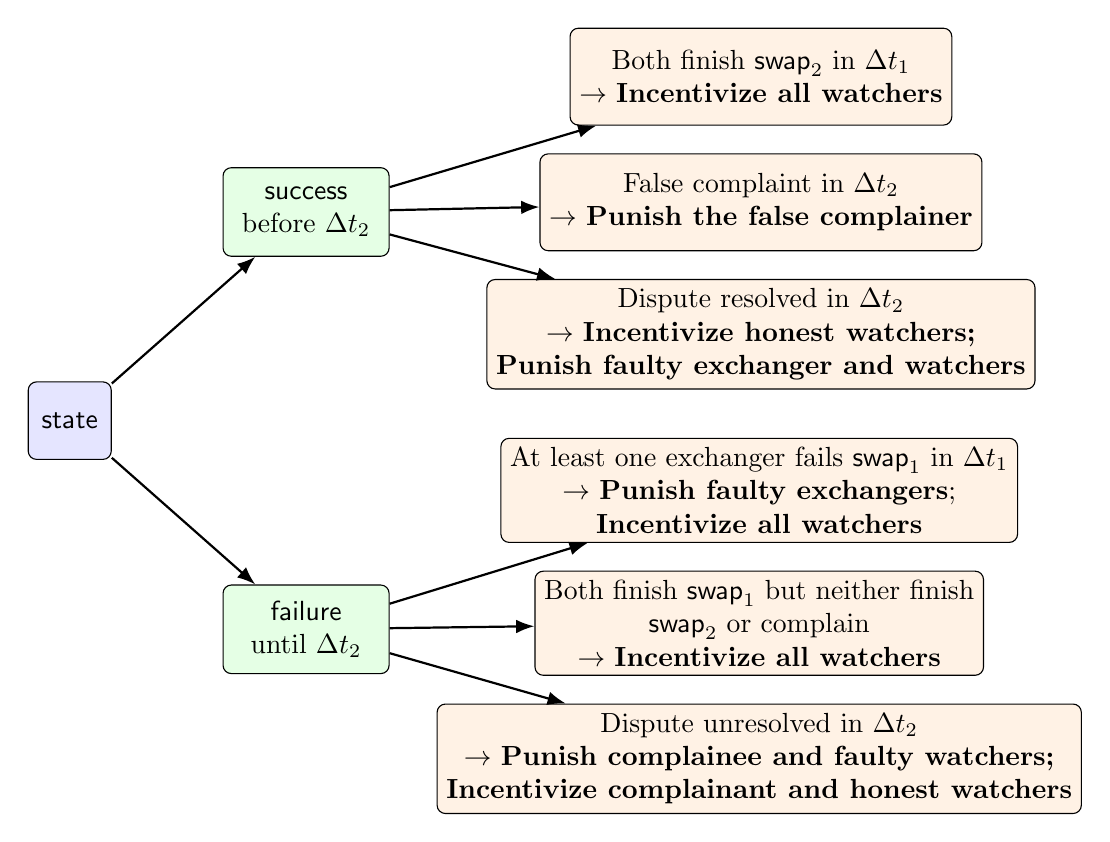
\begin{tikzpicture}[
    >=Latex,    
    node distance=1.8em and 4em, 
    root/.style={draw, rectangle, rounded corners=3pt, minimum width=3em, minimum height=2.8em, align=center, fill=blue!10},
    branch/.style={draw, rectangle, rounded corners=3pt, minimum width=6em, minimum height=3.2em, align=center, fill=green!10},
    leaf/.style={draw, rectangle, rounded corners=3pt, minimum width=10em, minimum height=3.5em, align=center, fill=orange!10},
    arrow/.style={->, line width=0.8pt}
]

% Root node
\node[root] (state) {$\mathsf{state}$};

% First level branches
\node[branch, above right=4.5em and 4em of state] (success) {$\mathsf{success}$ \\before $\Delta t_2$};
\node[branch, below right=4.5em and 4em of state] (failure) {$\mathsf{failure}$ \\until $\Delta t_2$};

\draw[arrow] (state) -- (success);
\draw[arrow] (state) -- (failure);

% Success branch leaves
\node[leaf, above right=1.5em and 6.5em of success] (s1) {Both finish $\mathsf{swap}_2$ in $\Delta t_1$\\$\rightarrow$ \textbf{Incentivize all watchers}};
\node[leaf, below=1em of s1] (s2) {False complaint in $\Delta t_2$\\$\rightarrow$ \textbf{Punish the false complainer}};
\node[leaf, below=1em of s2] (s3) {Dispute resolved in $\Delta t_2$\\$\rightarrow$ \textbf{Incentivize honest watchers;}\\  \textbf{Punish faulty exchanger and watchers}};


\draw[arrow] (success) -- (s1);
\draw[arrow] (success) -- (s2);
\draw[arrow] (success) -- (s3);

% Failure branch leaves
\node[leaf, above right=1.5em and 4em of failure] (f1) {At least one exchanger fails $\mathsf{swap}_1$ in $\Delta t_1$\\$\rightarrow$ \textbf{Punish faulty exchangers};\\ \textbf{Incentivize all watchers}};
\node[leaf, below=1em of f1] (f2) {Both finish $\mathsf{swap}_1$ but neither finish\\ $\mathsf{swap}_2$ or complain\\$\rightarrow$ \textbf{Incentivize all watchers}};
\node[leaf, below=1em of f2] (f3) {Dispute unresolved in $\Delta t_2$\\$\rightarrow$ \textbf{Punish complainee and faulty watchers;}\\ \textbf{Incentivize complainant and honest watchers}};

\draw[arrow] (failure) -- (f1);
\draw[arrow] (failure) -- (f2);
\draw[arrow] (failure) -- (f3);

\end{tikzpicture}
}
\caption{The incentive and penalty mechanism}
    \label{fig:incentive_mindmap}
\end{figure}

\subsubsection{Incentive Mechanism}
A swap instance ends with either $\success$ or $\failure$ definitely (proved by Lemma~\ref{lem:termination}). Specifically, the $\success$ can be determined before $\Delta t_2$ and the $\failure$ is determined only after $\Delta t_2$.
We assume that all entities are required to make stakes in the system; and the number of swap instances a watcher can serve simultaneously is proportional to the amount of its stakes.
Figure~\ref{fig:incentive_mindmap} presents the mindmap to illustrate all cases of results and the corresponding incentive policy a swap instance.


The $\success$ results include three cases. The first case is optimistic scenario where both exchangers honestly invoke $\mathsf{swap}_1$ and $\mathsf{swap}_2$ before $\Delta t_1$. In this case, the watchers are not involved and each of them is rewarded with a small tip. 
The second case introduces the scenario where some exchanger may propose false complaint. In this case, the complainer will be punished.
The third case shows the scenario where one exchanger does not execute $\mathsf{swap}_2$ before $\Delta t_2$. Then, the other exchanger notice the $n$ watchers to resolve the dispute. In this case, faulty exchanger and watchers are punished to reward the honest watchers who send $\mathsf{swap}_2$ before $\Delta t_2$.



The $\failure$ results also contains three cases. The first case means at least one exchangers give up in $\Delta t_1$. Hence, the faulty exchanger will be punished and all watchers are rewarded. The second case means both exchangers negotiate to abort the swap instance before $\Delta t_2$, then all watchers are rewarded. The third case is an unexpected scenario, where honest complaint is raised but unresolved due to insufficient honest watchers. We impose penalties on the complainee and faulty watchers to compensate the complainant and honest watchers.
\subsection{Security Properties}
\label{sec:security-properties}


We prove in Appendix~\ref{sec:uc-dex-security} that the real-world protocol $\Pi_{\mathsf{DEX}}$ UC-securely realizes the ideal functionality $\mathcal{F}_{\mathsf{DEX}}$ and the DEX $\Pi_{\mathsf{DEX}}$ guarantees the security properties by Lemmas~\ref{lem:decentralization}-\ref{lem:incentive}.
% Consequently, all security properties of $\Pi_{\mathsf{DEX}}$ follow directly from those of $\mathcal{F}_{\mathsf{DEX}}$.
% In particular, the following lemmas are immediate corollaries of the UC security guarantee:




\section{Experimental Evaluation}
\label{sec:experiments}
We implement our PVGSS scheme using Golang (off-chain) and Solidity (on-chain). The method in~\cite{Lewko2011DABE} supports only boolean formula-based access structures; therefore, we adopt the approach proposed in~\cite{Liu2010LSSS} to transform a general access structure into a LSSS matrix. To make on-chain and off-chain operations compatible, we choose BN128 as the asymmetric elliptic curve group, which is officially supported by Ethereum. 
% The on-chain exponentiation is about $40000$.\footnote{\url{https://eips.ethereum.org/EIPS/eip-196\#gas-costs}}
The benchmarks of PVGSS schemes are executed on a Intel (R) Core (TM) i7-11800H @2.30GHz with 4GB RAM running Ubuntu 22.04.5 LTS and Golang1.22.0. The smart contract codes are deployed and tested on Ethereum Sepolia testnet.
% The source code of contract is deployed and available on Ethereum Sepolia testnet.
% \footnote{\url{https://sepolia.etherscan.io/address/0xfc725a86fe14ee68b645f9d92e832b0d843045ee\#code}}. 
% The proof of concept implementation is available on GitHub\footnote{\url{https://github.com/scottocs/pvgss}}.


We choose the access structure designed for the DEX (cf. Figure~\ref{fig:swap_as}) to evaluate the performance of the PVGSS scheme, where $t=n/2+1$ and $n$ ranges from 100 to 1000. Figure~\ref{fig:pvgssShare_cost}-\ref{fig:pvgssRecon_cost} show the off-chain computational overheads of the PVGSS schemes. The cost of $\pvgssShare$ and $\pvgssRecon$ are super-linear, due to polynomial evaluation and Lagrange interpolation in Shamir SS-based approach and matrix multiplication in LSSS-based approach. Besides, the $\pvgssPreRecon$ algorithm costs about 418$\mu$s for calculation of each $K_i$. 
It can be seen all algorithms can be calculated within seconds given $n=1000$, indicating practicality of the PVGSS schemes in large-scale systems.

\begin{figure}[!htp]
    \begin{minipage}[c]{0.3\textwidth}
    \centering
    \scalebox{0.5}{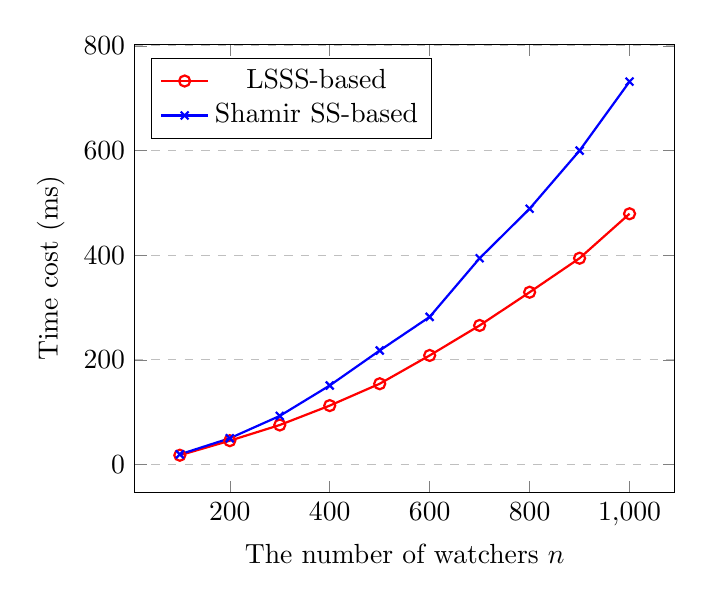
\begin{tikzpicture}[thick]
    \begin{axis}[
      xticklabel style={},
      legend style={at={(0.5,-0.35)},
      legend pos=north west,
      },
      ymajorgrids=true,
      grid style=dashed,
      xlabel=The number of watchers $n$,
      ylabel=Time cost (ms)
      ]
    
     \addplot[color=red,thick, mark=o]  coordinates{(100, 17.97) (200, 45.74) (300, 75.70) (400, 112.78) (500, 154.52) (600, 208.58) (700, 265.87) (800, 329.32) (900, 394.29) (1000, 479.20) };
     \addplot[color=blue,thick, mark=x]  coordinates{(100, 19.63) (200, 50.38) (300, 93.05) (400, 151.20) (500, 217.98) (600, 282.23) (700, 394.25) (800, 488.83) (900, 599.82) (1000, 731.60)};     
    % \addplot[color=white]  coordinates{(1, 1.8)};
    \legend{LSSS-based, Shamir SS-based}
    \end{axis}
    \end{tikzpicture}}
    \caption{Cost of $\pvgssShare$\label{fig:pvgssShare_cost}}
  \end{minipage}
  \begin{minipage}[c]{0.3\textwidth}
    \centering
    \scalebox{0.5}{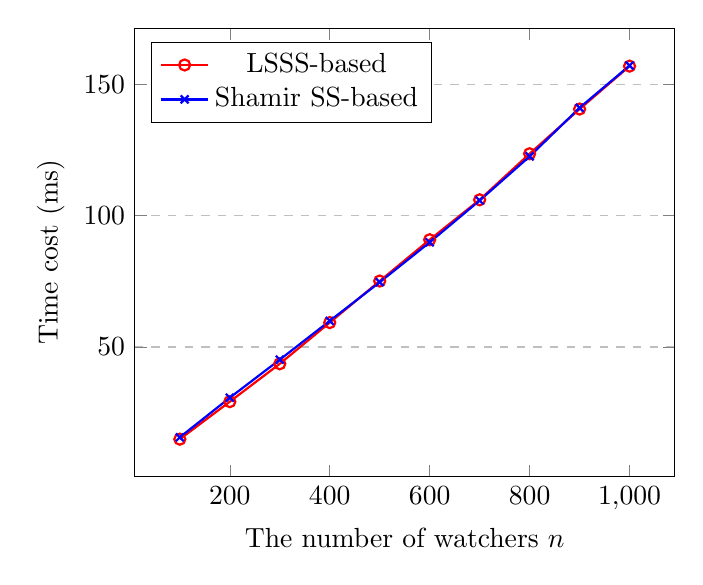
\begin{tikzpicture}[thick]
    \begin{axis}[
      xticklabel style={},
      legend style={at={(0.5,-0.35)},
      legend pos=north west,
      },
      ymajorgrids=true,
      grid style=dashed,
      xlabel=The number of watchers $n$,
      ylabel=Time cost (ms)
      ]
    
     \addplot[color=red,thick, mark=o]  coordinates{(100, 14.88) (200, 29.17) (300, 43.59) (400, 59.28) (500, 75.11) (600, 90.83) (700, 106.04) (800, 123.58) (900, 140.60) (1000, 156.94) };
     \addplot[color=blue,thick, mark=x]  coordinates{(100, 15.60) (200, 30.67) (300, 45.16) (400, 59.93) (500, 74.66) (600, 89.84) (700, 105.77) (800, 122.56) (900, 141.07) (1000, 157.15) };     
    % \addplot[color=white]  coordinates{(1, 1.8)};
    \legend{LSSS-based, Shamir SS-based}
    \end{axis}
    \end{tikzpicture}}
    \caption{Cost of $\pvgssVerify$ \label{fig:pvgssVerify_cost}}
  \end{minipage}
  \begin{minipage}[c]{0.3\textwidth}
    \centering
    \scalebox{0.5}{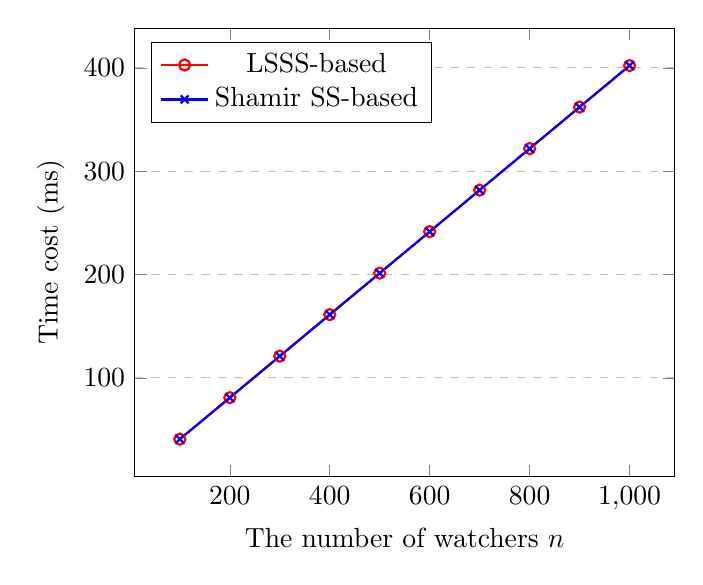
\begin{tikzpicture}[thick]
    \begin{axis}[
      xticklabel style={},
      legend style={at={(0.5,-0.35)},
      legend pos=north west,
      },
      ymajorgrids=true,
      grid style=dashed,
      xlabel=The number of watchers $n$,
      ylabel=Time cost (ms)
      ]
    
     \addplot[color=red,thick, mark=o]  coordinates{(100, 40.58) (200, 80.75) (300, 120.93) (400, 161.1) (500, 201.28) (600, 241.46) (700, 281.632) (800, 321.81) (900, 361.98) (1000, 402.16) };
     \addplot[color=blue,thick, mark=x]  coordinates{(100, 40.58) (200, 80.75) (300, 120.93) (400, 161.1) (500, 201.28) (600, 241.46) (700, 281.632) (800, 321.81) (900, 361.98) (1000, 402.16) };     
    % \addplot[color=white]  coordinates{(1, 1.8)};
    \legend{LSSS-based, Shamir SS-based}
    \end{axis}
    \end{tikzpicture}}
    \caption{Cost of $n$ times of $\pvgssKeyVrf$\label{fig:pvgssKeyVrf_cost}}
  \end{minipage}
\end{figure}
\begin{figure}[!htp]
  \begin{minipage}[c]{0.3\textwidth}
    \centering
    \scalebox{0.5}{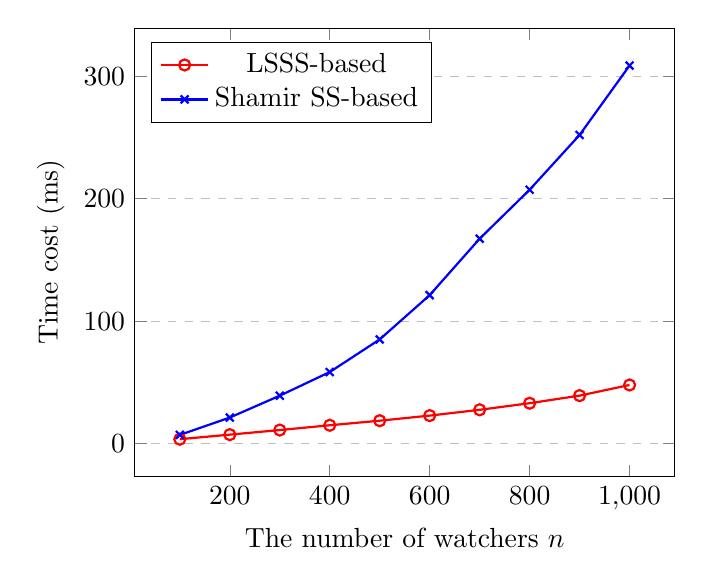
\begin{tikzpicture}[thick]
    \begin{axis}[
      xticklabel style={},
      legend style={at={(0.5,-0.35)},
      legend pos=north west,
      },
      ymajorgrids=true,
      grid style=dashed,
      xlabel=The number of watchers $n$,
      ylabel=Time cost (ms)
      ]
    
     \addplot[color=red,thick, mark=o]  coordinates{(100, 3.73) (200, 7.44) (300, 11.20) (400, 15.10) (500, 18.83) (600, 22.98) (700, 27.72) (800, 33.10) (900, 39.30) (1000, 47.99) };
     \addplot[color=blue,thick, mark=x]  coordinates{(100, 7.23) (200, 21.40) (300, 39.25) (400, 58.53) (500, 85.19) (600, 121.33) (700, 167.41) (800, 207.36) (900, 252.08) (1000, 308.73)};     
    % \addplot[color=white]  coordinates{(1, 1.8)};
    \legend{LSSS-based, Shamir SS-based}
    \end{axis}
    \end{tikzpicture}}
    \caption{$\pvgssRecon$ with an authorized set size $t+1$ \label{fig:pvgssRecon_cost}}
  \end{minipage}
  \begin{minipage}[c]{0.3\textwidth}
    \centering
    \scalebox{0.5}{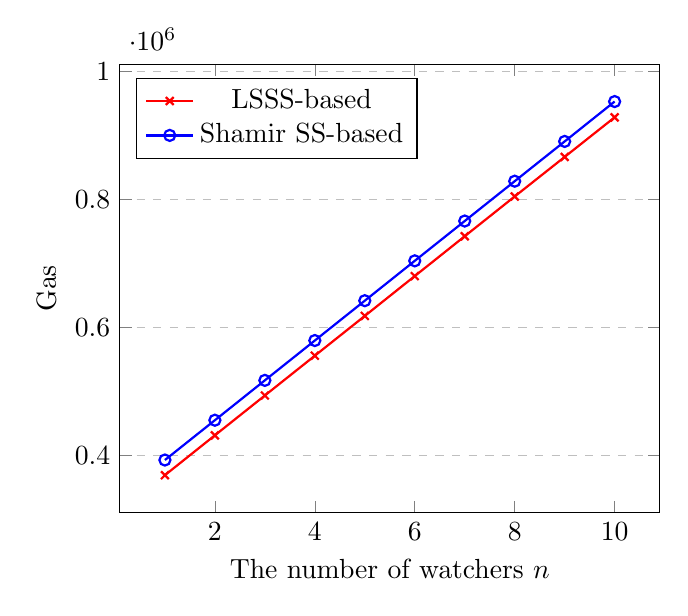
\begin{tikzpicture}[thick]
    \begin{axis}[
      xticklabel style={},
      legend style={at={(0.5,-0.35)},
      legend pos=north west,
      },
      ymajorgrids=true,
      grid style=dashed,
      xlabel=The number of watchers $n$,
      ylabel=Gas
      ]
    \addplot[color=red,thick, mark=x]  coordinates{(1,369131) (2,431397) (3,493655) (4,555845) (5,618039) (6,680345) (7,742608) (8,804779) (9,866611) (10,928511)};          
    \addplot[color=blue,thick, mark=o]  coordinates{(1, 392807) (2,  455029) (3,  517314) (4,  579604) (5,  641875) (6,  704161) (7,  766404) (8,  828663) (9,  890839) (10, 953155)};
     
    % \addplot[color=white]  coordinates{(1, 1.8)};
    \legend{LSSS-based, Shamir SS-based}
    \end{axis}
    \end{tikzpicture}}
    \caption{On-chain gas cost of $\mathsf{swap_1}+\mathsf{swap_2}$\label{fig:swap1_op}}
  \end{minipage}
  \begin{minipage}[c]{0.3\textwidth}
    \centering
    \scalebox{0.5}{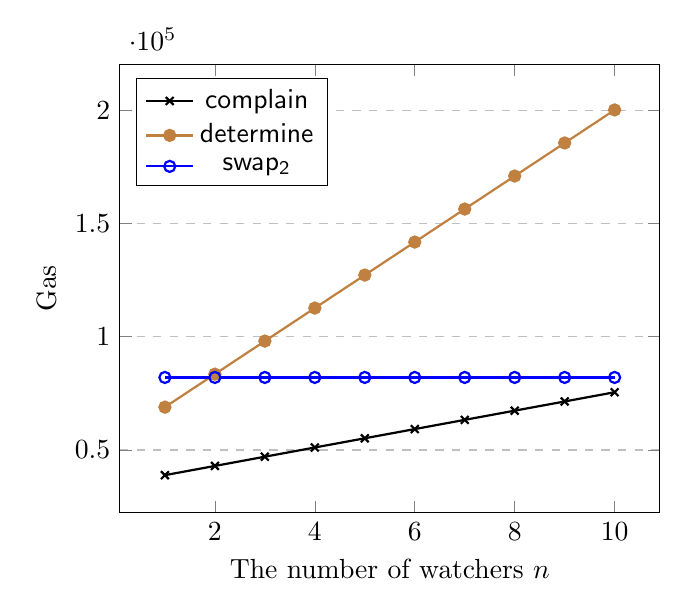
\begin{tikzpicture}[thick]
    \begin{axis}[
      xticklabel style={},
      legend style={at={(0.5,-0.35)},
      legend pos=north west,
      },
      ymajorgrids=true,
      grid style=dashed,
      xlabel=The number of watchers $n$,
      ylabel=Gas
      ]
    
     \addplot[color=black,thick, mark=x]  coordinates{(1, 38894) (2, 42959) (3, 47036) (4, 51101) (5, 55166) (6, 59231) (7, 63296) (8, 67361) (9, 71414) (10, 75491)};     
     \addplot[color=brown,thick, mark=*]  coordinates{(1, 68917) (2, 83487) (3, 98069) (4, 112639) (5, 127209) (6, 141779) (7, 156349) (8, 170919) (9, 185499) (10, 200081)};     
     \addplot[color=blue,thick, mark=o]  coordinates{(1, 82020) (2, 82020) (3, 82020) (4, 82020) (5, 82020) (6, 82020) (7, 82020) (8, 82020) (9, 82020) (10, 82020)};     
     \addplot[color=white,thick, mark=o]  coordinates{(1, 203784)};     
    \legend{$\mathsf{complain}$, $\mathsf{determine}$, $\mathsf{swap_2}$}
    \end{axis}
    \end{tikzpicture}}
    \caption{On-chain cost of $\mathsf{complain}$, $\mathsf{determine}$, $\mathsf{swap_2}$\label{fig:swap_complain_determin}}
  \end{minipage}
\end{figure}



% for x in [167767,71250,310787,559855,808882,82020,392807,641875,890839,38894,55166,71414,68917,127209,185499]: print("\$"+str(round(x*2958*0.206/1000000000, 3)));
\renewcommand{\arraystretch}{1.2} 
\begin{table}[!b]
    \centering
    \caption{Monetary cost of the on-chain operations\label{tab:monetary_cost}}
    \begin{tabular}{|c|cc|c|}
    \hline
    Operation&\multicolumn{2}{c|}{Gas cost}&USD\\\hline
    $\mathsf{register}$&\multicolumn{2}{c|}{167767}&\$0.102  \\\hline
    $\mathsf{freeze}$&\multicolumn{2}{c|}{71250}&\$0.043  \\\hline 
    \multirow{3}{*}{$\mathsf{swap_1}$} &$n$=1&310787&\$0.189   \\
    \cline{2-4}&$n$=5&559855&\$0.341 \\    
    \cline{2-4}&$n$=9&808882&\$0.493   \\\hline
    $\mathsf{swap_2}$&\multicolumn{2}{c|}{82020} &\$0.05  \\\hline
    \rowcolor{gray!30} \multirow{3}{*}{} \textbf{total}, i.e.,&$n$=1&392807&\$0.239 \\
    \cline{2-4}\rowcolor{gray!30}$\mathsf{swap_1}+\mathsf{swap_2}$&$n$=5&813639&\$0.391  \\
    \cline{2-4}\rowcolor{gray!30}(Shamir SS-based)&$n$=9&1062603&\$0.543 \\\hline
    \multirow{3}{*}{$\mathsf{complain}$} &$n$=1&38894&\$0.024  \\
    \cline{2-4}&$n$=5&55166&\$0.034   \\
    \cline{2-4}&$n$=9&71414&\$0.044   \\\hline
    \multirow{3}{*}{$\mathsf{determine}$} &$n$=1&68917&\$0.042   \\
    \cline{2-4}&$n$=5&127209&\$0.078  \\
    \cline{2-4}&$n$=9&185499&\$0.113   \\\hline
\end{tabular}
\end{table}


Further, we evaluate the gas consumption of the DEX. As proved in Lemma~\ref{lem:dos}, we can set $t=1$ and arbitrary $n\geq 1$ for the DEX in practice. We present the on-chain gas cost with $n$ ranging from $1$ to $10$.
We first introduce the cost in the normal case, where both exchangers honestly abide by the protocol.
In $\mathsf{swap_1}$, calculation of $\pvgssVerify$ and storage of $\{C_i\}$ are included. 
The $\mathsf{swap_2}$, which invokes $\pvgssKeyVrf$, roughly costs a constant amount gas (i.e., 82020) for each exchanger. 
The $\pvgssKeyVrf$ algorithm is the same for both LSSS-based and Shamir SS-based PVGSS, hence they cost equal gas consumption.
Figure~\ref{fig:swap1_op} depicts the gas consumption of the $\mathsf{swap_1}+\mathsf{swap_2}$ on smart contract.
It can be observed that the LSSS-based $\pvgssShare$ is slightly more efficient, as matrix multiplication is somewhat more computationally intensive than Lagrange interpolation in Solidity.
Then, we depict the gas cost in exceptional scenarios where arbitration procedures are required. Particularly, an exchanger calls $\mathsf{complain}$, then each watcher invokes $\mathsf{swap_2}$ and finally anyone can execute $\mathsf{determine}$.
Figure~\ref{fig:swap_complain_determin} shows the gas cost of functionalities of $\mathsf{complain}$, $\mathsf{determine}$ and $\mathsf{swap_2}$. 




% As of the time of writing (March 18, 2025), the median gas price is 1.1 gwei, and the price of ETH is 1,940 USD.
As of the time of writing (November 25, 2025), the median gas price is 0.206 gwei, and the price of ETH is 2,958 USD.\footnote{\url{https://etherscan.io/gastracker}}
Table~\ref{tab:monetary_cost} presents the monetary cost of each operation on the smart contract. For convenience, only the Shamir SS-based PVGSS is evaluated. The gray cells highlight the optimistic case, where the cost for each exchanger is only \$0.239/\$0.391/\$0.543 for $n$ = 1/5/9 and $t=1$.
If watchers are involved in the pessimistic case, the complaint cost is less than 0.044 USD, and each watcher incurs a cost of approximately 0.05 USD (as \(\mathsf{swap_2}\) requires).




% \section{Other Applications}



% publicly verifiable PRE with hierarchical organzied proxies
% Optimistic fair exchange/multiparty exchange 
% timelock contract/key escrow
% secure 2-party computation (2PC) protocol
% decentralied TTP/ token bridge/ distributed trust/ relay nodes or network/ Sidechains
% Voting/ DAO governance / https://arxiv.org/pdf/2310.19201
% Secret Multiple Leaders & Committee Election
% channel / multi-signature

\section{Conclusion}
\label{sec:conclusion}
We begin by introducing the concept of publicly verifiable generalized secret sharing (PVGSS) and compare it with other SS-related schemes (i.e., LSSS, GSS, VSS, PVSS and CPABE). The comparison highlights that PVGSS not only supports generalized access structure, but also facilitates public verifiability, making it ideal primitive for transparent systems like blockchain. Then we propose two constructions with unified description: one is Shamir-based and the other is LSSS-based.
Rigorous proofs are given to prove the security proofs of the constructions.
Furthermore, we build a PVGSS-based decentralized exchange (DEX), which guarantees optimistic fairness and passive arbitration due to the sophisticated designed access structure. Comprehensive experiments and detailed analysis demonstrates the feasibility of the DEX in real-world applications.
Looking ahead, we plan to further explore PVGSS-related research. First, we aim to implement additional applications discussed in Section~\ref{sec:other_applications} and beyond. Second, we intend to investigate more PVGSS constructions. Lastly, we will explore variations of PVGSS schemes, such as proactive PVGSS or q-PVGSS, akin to proactive SS~\cite{Bagherpour2022VPSS} and q-PVSS~\cite{cascudo2024publicly}.



% \newpage
\appendix
% \section{Access Structure Examples}
% \label{sec:as_examples}








\section{UC-Based Security of the DEX}
\label{sec:uc-dex-security}

In this appendix, we prove the security of the decentralized exchange protocol
$\Pi_{\mathsf{DEX}}$ in the Universal Composability (UC) framework~\cite{Canetti2000UC}.
Specifically, we show that $\Pi_{\mathsf{DEX}}$ securely realizes the ideal
functionality $\mathcal{F}_{\mathsf{DEX}}$ under static corruptions, assuming the
underlying PVGSS construction satisfies correctness, public verifiability, and IND1-secrecy (Theorems~\ref{theo:correctness}~--\ref{theo:ind1secrecy}).

\paragraph{Blockchain Model.}
We work in the UC hybrid model with a global ledger functionality $\mathcal{F}_{\mathsf{Ledger}}$, which maintains an append-only public state and executes smart contracts deterministically. The adversary controls transaction scheduling and message delivery, but cannot modify ledger state or contract code. This abstraction is standard in UC analyses of blockchain-based protocols. The global ledger functionality $\mathcal{F}_{\mathsf{Ledger}}$ maintains a public, append-only state.


\paragraph{Adversarial Model.}
We consider a probabilistic polynomial-time (PPT) adversary $\mathcal{A}$ that
statically corrupts a subset of parties before protocol execution. The
environment $\mathcal{Z}$ observes all public ledger events and interacts
arbitrarily with $\mathcal{A}$.

% \paragraph{Corruption Threshold.}
% We assume that fewer than $t$ watchers are corrupted, where $t$ is the reconstruction threshold of the PVGSS access structure. This assumption is required for the real-world protocol $\Pi_{\mathsf{DEX}}$ to securely realize the ideal functionality $\mathcal{F}_{\mathsf{DEX}}$. If the bound is violated, the real execution may leak information that no simulator can reproduce in the ideal world.


\paragraph{Proof System Assumptions.}
We assume that the NIZK proofs used in \textsf{PVGSSShare} are simulation-extractable in the Random Oracle Model (ROM). In particular, for any accepting proof generated by a corrupted party, there exists a PPT extractor that recovers a witness consistent with the statement. The DLEQ proofs used in \textsf{swap2} satisfy soundness and adaptive zero-knowledge.

% \subsection{Main Theorem}

% 替换原 Theorem A.1 为：
\begin{theorem}[UC Security of $\Pi_{\mathsf{DEX}}$]
\label{thm:uc-dex}
Assume the underlying PVGSS scheme satisfies correctness, public verifiability, and IND1-secrecy (Theorems~\ref{theo:correctness}–\ref{theo:ind1secrecy}).
Then, for any probabilistic polynomial-time (PPT) adversary $\mathcal{A}$ in the real world interacting with $\Pi_{\mathsf{DEX}}$ and $\mathcal{F}_{\mathsf{Ledger}}$,
there exists a PPT simulator $\mathcal{S}$ in the ideal world interacting only with $\mathcal{F}_{\mathsf{DEX}}$ and $\mathcal{F}_{\mathsf{Ledger}}$,
such that for all PPT environments $\mathcal{Z}$,
\[
    \mathsf{EXEC}_{\Pi_{\mathsf{DEX}}, \mathcal{A}, \mathcal{Z}} \approx_c \mathsf{EXEC}_{\mathcal{F}_{\mathsf{DEX}}, \mathcal{S}, \mathcal{Z}},
\]
where $\approx_c$ denotes computational indistinguishability.
\end{theorem}

% \begin{theorem}[UC Security of $\Pi_{\mathsf{DEX}}$]
% \label{thm:uc-dex}
% Assuming the above conditions, for any PPT real-world adversary $\mathcal{A}$
% interacting with $\Pi_{\mathsf{DEX}}$, there exists a PPT simulator $\mathcal{S}$
% such that for all PPT environments $\mathcal{Z}$,
% \[
% \mathsf{EXEC}_{\Pi_{\mathsf{DEX}}, \mathcal{A}, \mathcal{Z}}
% \;\approx_c\;
% \mathsf{EXEC}_{\mathcal{F}_{\mathsf{DEX}}, \mathcal{S}, \mathcal{Z}}.
% \]
% \end{theorem}

\subsection{Simulator Construction}

We construct a simulator $\mathcal{S}$ that interacts with $\mathcal{F}_{\mathsf{DEX}}$ and $\mathcal{F}_{\mathsf{Ledger}}$, while internally simulating the execution of $\Pi_{\mathsf{DEX}}$ for $\mathcal{A}$. 
The simulator internally emulates all interactions with $\mathcal{F}_{\mathsf{Ledger}}$, ensuring that the interface exposed to the environment is indistinguishable from that of the real ledger.

\textbf{Register.}
For each honest party, $\mathcal{S}$ samples a key pair
$(sk_i, pk_i) \leftarrow \textsf{PVGSSSetup}(\lambda)$ and registers $pk_i$ with
$\mathcal{F}_{\mathsf{DEX}}$. For corrupted parties, $\mathcal{S}$ forwards the
public keys chosen by $\mathcal{A}$. This distribution matches the real protocol.

\textbf{Deposit.}
Valid asset-freezing transactions submitted by $\mathcal{A}$ are forwarded to $\mathcal{F}_{\mathsf{DEX}}$ via $\mathcal{F}_{\mathsf{Ledger}}$. Invalid requests
are rejected, exactly as in the real-world execution.

\textbf{Commit (swap1).}
Upon receiving a commitment message
$(\textsf{swap1},$\\$id, \{C_i\}, \pi_s)$:

\begin{itemize}
  \item \emph{from corrupted exchanger}, 
    $\mathcal{S}$ invokes the knowledge extractor guaranteed by the simulation-extractability of the NIZK proof system used in $\pvgssShare$ (see Section~\ref{sec:sigma_protocol} and Theorem~\ref{theo:ver_enc_shares}).
  If extraction fails, $\mathcal{S}$ simulates contract rejection. Otherwise, $\mathcal{S}$ forwards the extracted information to $\mathcal{F}_{\mathsf{DEX}}$.

  \item \emph{from each honest party $i$}, $\mathcal{S}$ samples internal exponents $\alpha_i \xleftarrow{R} \mathbb{Z}_q$ and computes simulated ciphertexts $C_i = \textsf{pk}_i^0 \cdot g^{\alpha_i} = g^{\alpha_i}$. The simulator then invokes the zero-knowledge simulator $\mathcal{S}_{\text{PVGSS}}$ for the PVGSS NIZK proof system to generate $\pi_s \leftarrow \mathcal{S}_{\text{PVGSS}}(\{C_i\}, \mathbb{A})$. By the zero-knowledge property of the underlying proof system, the tuple $(\{C_i\}, \pi_s)$ is computationally indistinguishable from a valid commitment generated by an honest dealer in the real protocol.
\end{itemize}

\textbf{Reveal (swap2).}
When a decrypted share $(K_i, \pi_{K_i})$ is submitted:

\begin{itemize}
  \item \emph{For corrupted parties}, $\mathcal{S}$ verifies correctness using
  \textsf{PVGSSKeyVrf} and updates the state of $\mathcal{F}_{\mathsf{DEX}}$
  accordingly.

  \item \emph{For honest party $i$}, $\mathcal{S}$ computes $K_i = g^{\alpha_i}$ where $\alpha_i \in \mathbb{Z}_q$ is the internal exponent previously used to generate the simulated commitment $C_i = \textsf{pk}_i^0 \cdot g^{\alpha_i}$ during the \textbf{commit (swap1)} phase. Subsequently, $\mathcal{S}$ invokes the adaptive zero-knowledge simulator $\mathcal{S}_{\text{DLEQ}}$ for the DLEQ proof system to generate $\pi_{K_i} \leftarrow \mathcal{S}_{\text{DLEQ}}(C_i, K_i, g, \textsf{pk}_i,\alpha_i)$, demonstrating algebraic consistency between $C_i$ and $K_i$ without knowledge of any actual protocol secret share.
\end{itemize}



\textbf{Complain.}
If $\mathcal{A}$ invokes a complaint after deadline $\Delta t_1$, $\mathcal{S}$ forwards it to $\mathcal{F}_{\mathsf{DEX}}$. 

\textbf{Determine.}
Upon determination, $\mathcal{S}$ queries $\mathcal{F}_{\mathsf{DEX}}$ and reproduces the outcome (\textsf{success} or \textsf{failure}) on the simulated ledger, including asset transfers and penalties.


\begin{theorem}[Simulation Consistency]\label{the:consistency}
The simulator maintains internal state to ensure algebraic consistency between simulated commitments and simulated reveals. In particular, the PVGSS encryption scheme supports programmable ciphertexts, ensuring that simulated ciphertexts in \textbf{commit (swap1)} phase and simulated decrypted shares in \textbf{Reveal (swap2)} remain mutually consistent.
\end{theorem}
% \paragraph{Simulation Consistency.}

\subsection{Indistinguishability Argument}

All information observable by the environment $\calZ$ is either derived from the public ledger state or from messages sent by corrupted parties. By Theorem~\ref{the:consistency}, the simulator $\mathcal{S}$ exactly emulates the ledger interface, smart contract logic, and the behavior of corrupted parties. Hence, any difference between the real and ideal executions can only arise from the simulation of honest-party cryptographic messages. We define a sequence of hybrid games to bound this difference.

\begin{itemize}
    \item \textbf{Hybrid 0 (Real):} The actual execution of $\Pi_{\text{DEX}}$ with $\adv$.
    \item \textbf{Hybrid 1 (Simulation of Honest Proofs):} Replace real NIZK proofs (PVGSSShare and DLEQ) generated by honest parties with simulated proofs.
    \emph{Indistinguishability:} Follows from the \textbf{Zero-Knowledge} property of the underlying Sigma protocols and DLEQ proofs.
    \item \textbf{Hybrid 2 (Simulation of Ciphertexts):} Replace honest commitments $C = \text{Enc}(pk, s)$ with $C^* = \text{Enc}(pk, 0)$.
    \emph{Indistinguishability:} Follows from the \textbf{IND1-secrecy} of PVGSS (Theorem~\ref{theo:ind1secrecy}). Since $\adv$ controls an unauthorized set during the commitment phase, the ciphertexts reveal no information about the secret.
    \item \textbf{Hybrid 3 (Extraction):} For corrupted parties, $\mathcal{S}$ extracts witnesses using the ROM programmability.
    \emph{Indistinguishability:} Follows from the \textbf{Soundness} of the NIZK proofs. If $\adv$ produces a valid proof without a valid witness, it breaks soundness.
    \item \textbf{Hybrid 4 (Ideal):} $\mathcal{S}$ uses the extracted/simulated values to interact with $\dex$. The ledger state is updated exactly as $\dex$ dictates.
\end{itemize}

Summarily, the simulated execution is computationally indistinguishable from the real one due to the following properties:
\begin{itemize}
    \item \textbf{Zero-knowledge simulation.} The underlying NIZK proof systems---namely (i) the Sigma protocol with Fiat--Shamir transformation used in $\pvgssShare$, and (ii) the DLEQ proof used in $\pvgssPreRecon$---admit efficient simulators. This allows $\mathcal{S}$ to generate commitments and reveal messages for honest parties that are computationally indistinguishable from those in a real execution, while maintaining algebraic consistency.
    \item \textbf{IND1-secrecy of PVGSS.} By Theorem~\ref{theo:ind1secrecy}, the ciphertexts generated in the commitment phase are indistinguishable from encryptions of any other value to parties outside the authorized access structure. This ensures that the simulated ciphertexts used by $\mathcal{S}$ cannot be distinguished from real ones by $\adv$ or $\calZ$.
    \item \textbf{Soundness of verification.} The soundness of the PVGSS verification algorithms (Theorems~\ref{theo:ver_enc_shares} and~\ref{theo:ver_share_dec}) guarantees that any malformed commitments or decrypted shares submitted by $\adv$ are rejected with the same probability in both the real and ideal executions, ensuring identical acceptance and rejection behavior.
\end{itemize}

A standard hybrid argument over these components implies that the joint view of $\calZ$ and $\adv$ in the simulated execution is computationally indistinguishable from that in the real execution.


\subsection{Security Properties of the DEX}
\begin{lemma}[Decentralization]
\label{lem:decentralization}
Protocol $\Pi_{\mathsf{DEX}}$ is fully decentralized and does not rely on
any trusted third party.
\end{lemma}

\begin{proof}
Any party can permissionlessly register on-chain as an exchanger or a watcher
by depositing the required assets. All protocol logic---including commitment,
verification, secret reconstruction, arbitration, and settlement---is executed
by smart contracts together with publicly verifiable cryptographic algorithms.
No trusted coordinator, manager, or key holder is assumed at any stage of the
protocol. Hence, $\Pi_{\mathsf{DEX}}$ is decentralized by design.
\end{proof}

\begin{lemma}[Termination]\label{lem:termination}
\label{lem:termination}
Every execution of $\Pi_{\mathsf{DEX}}$ terminates within a bounded time.
\end{lemma}

\begin{proof}
The protocol enforces two explicit deadlines $\Delta t_1 < \Delta t_2$.
If the required secrets are reconstructed before $\Delta t_1$, the session
terminates successfully. Otherwise, the smart contract deterministically
finalizes the session at time $\Delta t_2$ and refunds the frozen assets.
This behavior exactly matches the termination semantics of
$\mathcal{F}_{\mathsf{DEX}}$, guaranteeing termination regardless of adversarial
behavior.
\end{proof}

\begin{lemma}[Optimistic Fairness]\label{lem:fairness}
\label{lem:fairness}
Protocol $\Pi_{\mathsf{DEX}}$ guarantees fairness: an honest exchanger either
obtains the correct counterparty assets or is refunded.
\end{lemma}

\begin{proof}
Optimistic fairness follows from the following facts.
\begin{itemize}
  \item \emph{Binding commitments.} Before any asset transfer, both exchangers
  must publish PVGSS commitments via \textsf{PVGSSShare}, which are publicly
  validated by \textsf{PVGSSVerify}. Invalid commitments are rejected on-chain.

  \item \emph{Controlled secret release.} An honest exchanger can learn the
  counterparty's secret only if the counterparty reveals it honestly, or if at
  least $t$ watchers reconstruct the missing secret via
  \textsf{PVGSSRecon}. By the correctness of PVGSS (Theorem~\ref{theo:correctness}), any reconstructed
  secret is valid, triggering a successful atomic exchange.

  \item \emph{Detectable deviations.} Invalid encrypted shares in \textsf{swap1}
  are rejected by \textsf{PVGSSVerify} (Theorem~\ref{theo:ver_enc_shares}), and invalid decrypted shares in
  \textsf{swap2} are rejected by \textsf{PVGSSKeyVrf} (Theorem~\ref{theo:ver_share_dec}). If arbitration
  fails, dishonest parties are penalized and honest exchangers are refunded.
\end{itemize}
Therefore, an honest exchanger is never worse off.
\end{proof}

\begin{lemma}[Accountable Exchangers]\label{lem:accountable_exchangers}
\label{lem:accountable-exchangers}
Any dishonest behavior by an exchanger is publicly detectable.
\end{lemma}

\begin{proof}
In the commitment phase, exchanger accountability is enforced by the public
verifiability of encrypted shares via \textsf{PVGSSVerify} (Theorem~\ref{theo:ver_enc_shares}). In the
reveal phase, correctness of decrypted shares is enforced by
\textsf{PVGSSKeyVrf} and the soundness of the underlying DLEQ proofs
(Theorem~\ref{theo:ver_share_dec}). Hence, exchangers cannot deviate without detection.
\end{proof}

\begin{lemma}[Accountable Arbitration]\label{lem:accountable_watchers}
\label{lem:accountable-arbitration}
All arbitration actions performed by watchers are publicly verifiable and
accountable.
\end{lemma}

\begin{proof}
Upon a complaint, watchers submit decrypted shares together with verifiable
proofs generated by \textsf{PVGSSPreRecon}. These submissions are publicly
checked by \textsf{PVGSSKeyVrf}, ensuring that any incorrect arbitration behavior
is detected.
\end{proof}

\begin{lemma}[Optimistic and Stateless Arbitration]
\label{lem:optimistic}
Protocol $\Pi_{\mathsf{DEX}}$ supports optimistic and stateless arbitration.
\end{lemma}

\begin{proof}
If both exchangers are honest, the access structure guarantees that secrets can
be reconstructed before $\Delta t_1$ without involving watchers, demonstrating
optimism. Watchers participate only upon explicit complaints and rely solely on
on-chain information, maintaining no local state for individual sessions.
\end{proof}

\begin{lemma}[Incentive Compatibility]
\label{lem:incentive}
$\Pi_{\mathsf{DEX}}$ admits incentive-compatible mechanisms that encourage honest
behavior.
\end{lemma}

\begin{proof}
By Lemmas~\ref{lem:accountable-exchangers} and
\ref{lem:accountable-arbitration}, all deviations are detectable. This enables
the protocol to reward honest behavior and penalize misbehavior through deposits
and slashing, making honest participation a rational strategy.
\end{proof}


Given the above lemmas, we argue that the following potential threats to the DEX have minimal impact.


\begin{myClaim}[Dos attack]\label{lem:dos}
Any DoS attack resulting in \(\failure\) termination can be detected (by Lemma~\ref{lem:accountable_exchangers} and Lemma~\ref{lem:accountable_watchers}), and the perpetrator will be penalized to compensate the victim using its deposited tokens.\qed
\end{myClaim}


\begin{myClaim}[Collusion/Coercion attack]\label{lem:collusion}
Owing to the transparency, availability, public accountability of smart contracts, an exchanger cannot obtain any advantage or compromise fairness, even when colluding with watchers.\qed
\end{myClaim}

\begin{myClaim}[Sybil attack]\label{lem:sybil}
An arbitrageur can be selected as a watcher in proportion to the amount of currency they have deposited. This implies that the nothing-at-stake attack is also eliminated. If a swap instance is ongoing, a proportional amount of deposited currency is locked, rendering a Sybil attack meaningless.\qed
\end{myClaim}

\begin{myClaim}[Rushing attack]\label{lem:rushing}
Rushing watchers, who attempt to gain benefits by providing arbitration without assistance from exchangers, make a futile attempt, as the honest exchangers incur no loss when following the protocol correctly.\qed
\end{myClaim}



\onecolumn

\section{Decisional Diffie-Hellman (DDH) Assumption}
The Decisional Diffie-Hellman (DDH)~\cite{Cascudo2017PVSS} assumption states that $(g, g^a, g^b, g^{ab})$ and $(g, g^a, g^b, g^c)$ are computationally indistinguishable, where $a, b, c \xleftarrow{R} \ZZ_q$ are chosen uniformly at random.
Formally, for any probabilistic polynomial-time (PPT) adversary $\adv$, the advantage of $\adv$ in distinguishing between the two distributions is negligible:
\[
\left| \Pr\left[\adv(g, g^a, g^b, g^{ab}) = 1\right] - \Pr\left[\adv(g, g^a, g^b, g^c) = 1\right] \right| \leq \mathsf{negl}(\lambda),
\]
where $\lambda$ is the security parameter, and $\mathsf{negl}(\lambda)$ denotes a negligible function in $\lambda$.



\section{Formal Definition of Security Properties for PVGSS}
\label{sec:pvgss_properties}
\begin{definition}[Correctness]\label{def:Correctness}
    The PVGSS is correct if for all authorized set $Q$ of $\mathbb{A}$, each $s$ in the secret space,
    { \[
    \Pr\left[
    \begin{aligned}
        &\pvgssVerify\left( \{C_i\}, \proofs_s, \mathbb{A} \right) = 1 \ \land \\
        &\pvgssKeyVrf(C_i, S_i, \proofs_{S_i}, \pk_i) = 1, \forall i \in I_{Q} \ \land \\ 
        & S' = g^s
    \end{aligned}
        \middle|
    \begin{aligned}
        &(\sk_i,\pk_i)\gets \pvgssSetup(\lambda); \\
        &(\{C_i\}, \proofs_s)\gets \pvgssShare(\mathbb{A}, \{\textsf{pk}_i\}) \\
        &\forall i \in I_{Q},(S_i, \proofs_{S_i}) \gets \pvgssPreRecon(C_i, \sk_i) \\
        &(S') \gets \pvgssRecon(\mathbb{A},Q);
    \end{aligned} 
    \right]
    =1\]}
\end{definition}

\begin{definition}[Verifiability of Encrypted Shares]\label{def:Ver_enc_share} 
    The PVGSS satisfies verifiability of encrypted shares if for every PPT $\adv$,
    { \[
    \Pr\left[ 
    \begin{aligned}
      &\pvgssVerify\left( \{C_i\}, \proofs_s, \mathbb{A} \right) = 1 \land \\
    & \nexists s \in S \ \text{s.t.} \ (\{C_i\}_{i \in [n]}, *) \gets \pvgssShare(\mathbb{A}, \{\pk_i\})\\    
    \end{aligned}
        \middle|
    \begin{aligned}
    &(\{\pk_i\}, \{\sk_i\}) \gets \pvgssSetup(\lambda), \\
    &(\{C_i\}, \proofs_s,\mathbb{A}) \gets \adv(\{\pk_i\})
    \end{aligned}
    \right]
    \leq negl(\lambda)\]}
\end{definition}

\begin{definition}[Verifiability of Share Decryption]\label{def:Ver_dec_share} 
    The PVGSS satisfies verifiability of share decryption if for every PPT $\adv$,
    { \[
    \Pr\left[ 
    \begin{aligned}
    &\pvgssKeyVrf(C, S, \proofs_{S}, pk) = 1 \land \\
    & \nexists sk \in  \{\sk_i\} \ \text{s.t.} \ (S, \proofs_{S}) \gets \pvgssPreRecon(C, sk)\\
    \end{aligned}
        \middle|
    \begin{aligned}
    &(\{\pk_i\}, \{\sk_i\}) \gets \pvgssSetup(\lambda), \\
    &(pk,C,S) \gets \adv(\{\pk_i\}), \ pk \in \{\pk_i\} 
    \end{aligned}
    \right]
    \leq negl(\lambda)\]}
\end{definition}


\begin{definition}[IND1-secrecy]\label{def:ind1secrecy}
    \textbf{IND1-secrecy} standards for indistinguishability of secrets. PVGSS achieves \textbf{IND1-secrecy} if for any polynomial time adversary $\adv$ without an authorized set, $\adv$ win the following game played against a challenger with negligible advantage.
    \begin{enumerate}        
        % TODO corrupted share or shareholder
        \item The challenger initiates the $\pvgssSetup$ algorithm for all honest parties and publishes the public keys $\{\pk_i\}$.
        \item $\adv$ generates a challenge access structure $\mathbb{A}^*$. $\adv$ chooses a maximum set of indexes $U\subset [1,\cdots, |\mathbb{A}^*|]$, where the shares corresponding to $U$ do not satisfy the access structure $\mathbb{A}^*$. It sends $\mathbb{A}^*, U$ to the challenger.
        \item The challenger randomly selects values $x_0$ and $x_1$ from the secret space. It then randomly selects $b \in \{0,1\}$. Further, it invokes $(\{C^*_i\},\proofs_{x_0}) \gets \pvgssShare(\mathbb{A}^*,\{\pk_i\})$, which indicates that $x_0$ is used as the secret. The challenger sends $(\{C^*_i\},\proofs_{x_0},x_b)$ to $\adv$.
        % \item The $\adv$ queries decrypted shares $\{S^*_i\}$ from the challenger who invokes $\pvgssPreRecon(C^*_i, \sk_i)$, as long as $\{S^*_i\}$ do not satisfy the access structure $\mathbb{A}^*$.
        \item $\adv$ then outputs a guess $b' \in \{0,1\}$.
    \end{enumerate}
    The $\adv$'s advantage in the game is defined as $|Pr[b = b'] - \frac{1}{2}|$.
\end{definition}

% \section{Global States in $\dex$}
% \label{sec:structs_global_states}
% \begin{lstlisting}
% struct Order {
%     address seller;    //Order creator
%     address tokenSell; //Token to sell (e.g., ETH)
%     uint256 amountSell; //Amount to sell (e.g., 2 ETH)
%     address tokenBuy; //Token to buy (e.g., USDT)
%     uint256 amountBuy; //Amount to buy (e.g., 7000 USDT)
%     bool isActive;     //Order state
% }
% // Store orders
% mapping(uint256 => Order) public orders;

% // values to track session state
% enum SessionState { Active, halfSwap1, finishSwap1, halfSwap2, Complain, Success, Failure }
% struct Session {
%     SessionState state; // Session state
%     address[] exchangers; // seller as exchanger[0], buyer as exchanger[1] in the session
%     address[] watchers; // Watchers in the session
%     mapping(address => G1Point) Cshares1; //shares from seller
%     mapping(address => G1Point) Cshares2; //shares from buyer
%     mapping(address => G1Point) shares;   //decrypted shares
%     uint256 t1; // Expiration time t1
%     uint256 t2; // Expiration time t2
%     bool[2] seller_flag; // swap flag of seller
%     bool[2] buyer_flag;  // swap flag of buyer
%     mapping(address => bool) watcher_flag; //submit flag of watcher
% }
% // Store sessions
% mapping(uint256 => Session) public sessions;

% //Events in the smart contract
% event TokensReceived(address token, address from, uint256 amount);
% event TokensFrozen(address token, address from, uint256 amount, uint256 sessionId);
% event TokensSwapped(address token, address from, uint256 amount, uint256 sessionId);
% event ComplaintFired(address complainer, uint256 sessionId);
% event SessionStateUpdated(uint256 sessionId, SessionState state);
% event UserNotified(uint256 sessionId, address user);
% event OrderCreated(uint256 orderId, address seller, address tokenSell, uint256 amountSell, address tokenBuy, uint256 amountBuy);
% event SessionCreated(uint256 orderId, address seller, address buyer, address[] watchers, uint256 t1, uint256 t2);
% event Incentivized(address user, uint256 amount);
% event Penalized(address user, uint256 amount);

% \end{lstlisting}




\bibliographystyle{plain}
\begin{thebibliography}{00}

\bibitem{Shamir79SS} Shamir, A. How to share a secret. \textit{Comm. of the ACM}, 1979, 22(11), pp. 612-613.

\bibitem{Das2022DKG}Das, S., Yurek, T., Xiang, Z., Miller, A., Kokoris-Kogias, L. and Ren, L. Practical asynchronous distributed key generation. In \textit{S\&P}, 2022, pp. 2518-2534.

\bibitem{Choi2023Beacon}Choi, K., Manoj, A. and Bonneau, J. Sok: Distributed randomness beacons. In \textit{S\&P}, 2023, pp. 75-92.

\bibitem{Syta2017Beacon}Syta, E., Jovanovic, P., Kogias, E.K., Gailly, N., Gasser, L., Khoffi, I., Fischer, M.J. and Ford, B. Scalable bias-resistant distributed randomness.In \textit{S\&P},2017, pp. 444-460.

\bibitem{Schindler2020Beacon}Schindler, P., Judmayer, A., Stifter, N. and Weippl, E., 2020, May. Hydrand: Efficient continuous distributed randomness. In 2020 IEEE Symposium on Security and Privacy (SP) (pp. 73-89). IEEE.



\bibitem{sahai2005fuzzy} Sahai, A., and Waters, B. Fuzzy identity-based encryption. In \textit{Eurocrypt}, 2005, pp. 457-473.


% \bibitem{Rathee2023Elsa}Rathee, M., Shen, C., Wagh, S. and Popa, R.A. Elsa: Secure aggregation for federated learning with malicious actors. In \textit{S\&P}, 2023, pp. 1961-1979.


% \bibitem{Dauterman2022Waldo}Dauterman, E., Rathee, M., Popa, R.A. and Stoica, I. Waldo: A private time-series database from function secret sharing. In \textit{S\&P}, 2022, pp. 2450-2468.

% \bibitem{Feneuil2023MPC}Feneuil, T. and Rivain, M. Threshold linear secret sharing to the rescue of MPC-in-the-head. In \textit{Asiacrypt}, 2023, pp. 441-473.


% \bibitem{Basu2019BFT}Basu, S., Tomescu, A., Abraham, I., Malkhi, D., Reiter, M.K. and Sirer, E.G. Efficient verifiable secret sharing with share recovery in BFT protocols. In \textit{CCS}, 2019, pp. 2387-2402.

\bibitem{Karchmer1993LSSS}Karchmer, M. and Wigderson, A. On span programs. In \textit{Annual Structure in Complexity Theory Conference}, 1993, pp. 102-111.


\bibitem{Feldman1987VSS} Feldman, P. A practical scheme for non-interactive verifiable secret sharing. In \textit{FOCS}, 1987, pp. 427-438.


\bibitem{Zhang2024VSS}Zhang, Z., Li, W., Guo, Y., Shi, K., Chow, S.S., Liu, X. and Dong, J. Fast {RS-IOP} Multivariate Polynomial Commitments and Verifiable Secret Sharing. In \textit{USENIX Security}, 2024, pp. 3187-3204.

\bibitem{cascudo2024publicly} Cascudo, I., and David, B. Publicly verifiable secret sharing over class groups and applications to DKG and YOSO. In \textit{Eurocrypt}, 2024, pp. 216-248.

\bibitem{Cascudo2017PVSS} Cascudo, I., and David, B. SCRAPE: Scalable randomness attested by public entities. In \textit{ACNS}, 2017, pp. 537-556.

% \bibitem{Massey1993DC}Massey, J.L. Minimal codewords and secret sharing. In \textit{the 6th joint Swedish-Russian international workshop on information theory}, 1993, pp. 276-279.

% \bibitem{Yuan2006DC}Yuan, J. and Ding, C. Secret sharing schemes from three classes of linear codes. \textit{IEEE transactions on information theory}, 2006, 52(1), pp.206-212.

\bibitem{Kate2010VSS}Kate, A., Zaverucha, G.M. and Goldberg, I., Constant-size commitments to polynomials and their applications. In \textit{Asiacrypt}, 2010, pp. 177-194.

\bibitem{Abraham2023VSS}Abraham, I., Jovanovic, P., Maller, M., Meiklejohn, S. and Stern, G. Bingo: Adaptivity and asynchrony in verifiable secret sharing and distributed key generation. In \textit{Crypto}, 2023, pp. 39-70.


\bibitem{Stadler1996PVSS} Stadler, M. Publicly verifiable secret sharing. In \textit{Eurocrypt}, 1996, pp. 190-199.

\bibitem{Ito1987GSS}Ito, M., Saito, A. and Nishizeki, T. Secret sharing scheme realizing general access structure. \textit{Electronics and Communications in Japan}, 1989, 72(9), pp. 56-64.

\bibitem{benaloh1990generalized} Benaloh, J., and Leichter, J. Generalized secret sharing and monotone functions. In \textit{Crypto}, 1990.

% \bibitem{Yu2010GAS}Yu, S., Wang, C., Ren, K. and Lou, W. Achieving secure, scalable, and fine-grained data access control in cloud computing. In \textit{INFOCOM}, 2010, pp. 1-9.

% \bibitem{Xu2018GAS}Xu, S., Yang, G., Mu, Y. and Deng, R.H. Secure fine-grained access control and data sharing for dynamic groups in the cloud. \textit{IEEE TIFS}, 2018, 13(8), pp. 2101-2113.

\bibitem{Garg2023MPC}Garg, S., Jain, A., Mukherjee, P., Sinha, R., Wang, M. and Zhang, Y. Cryptography with weights: MPC, encryption and signatures. In \textit{CRYPTO}, 2023, pp. 295-327.

\bibitem{Cao2025Web3}Cao, B., Xiao, S., Shi, L., Wang, T., Chen, J., Wang, J., Ling, X., Xu, H., Zhang, S. and Liu, E. Web 3.0: A survey on the architectures, enabling technologies, applications, and challenges. \textit{IEEE Communications Surveys \& Tutorials}, 2025.


% \bibitem{Solanki2018RAC}Solanki, N., Huang, Y., Yen, I.L., Bastani, F. and Zhang, Y. Resource and role hierarchy based access control for resourceful systems. In \textit{COMPSAC}, pp. 480-486.


\bibitem{Bethencourt2007CPABE} Bethencourt, J., Sahai, A., and Waters, B. Ciphertext-Policy Attribute-Based Encryption. In \textit{S\&P}, 2007, pp. 321-334.

\bibitem{Lewko2011DABE} Lewko, A., and Waters, B. Decentralizing attribute-based encryption. In \textit{Eurocrypt}, 2011, pp. 568-588.

\bibitem{Lin2018PVMSS}Lin, C., Hu, H., Chang, C.C. and Tang, S. A publicly verifiable multi-secret sharing scheme with outsourcing secret reconstruction. \textit{IEEE Access}, 2018, 6, pp. 70666-70673.

\bibitem{Beimel2025GSS}Beimel, A. Secret-Sharing Schemes for General Access Structures: An Introduction. \textit{Cryptology ePrint Archive}. 2025.

% \bibitem{Herranz2003VGSS}Herranz, J. and Sáez, G. Verifiable secret sharing for general access structures, with application to fully distributed proxy signatures. In \textit{FC}, 2003.

% \bibitem{Huber2022Voting}Huber, N., Küsters, R., Krips, T., Liedtke, J., Müller, J., Rausch, D., Reisert, P. and Vogt, A. Kryvos: Publicly tally-hiding verifiable e-voting. In \textit{CCS}, 2019, pp. 1443-1457.

% \bibitem{Baum2020MPC}Baum, C., Orsini, E., Scholl, P. and Soria-Vazquez, E. Efficient constant-round MPC with identifiable abort and public verifiability. In \textit{Crypto}, 2020, pp. 562-592.

% \bibitem{Parno2012VABE}Parno, B., Raykova, M. and Vaikuntanathan, V., 2012, March. How to delegate and verify in public: Verifiable computation from attribute-based encryption. In \textit{TCC}, 2012, pp. 422-439.


% \bibitem{Scafuro2019Blockchain}Scafuro, A., Siniscalchi, L. and Visconti, I. Publicly verifiable proofs from blockchains. In \textit{PKC}, 2019, pp. 374-401.

% \bibitem{Szydlo2004Merkle}Szydlo, M., 2004. Merkle tree traversal in log space and time. In \textit{Eurocrypt}, 2004, pp. 541-554.

% \bibitem{Kemmoe2024Acc}Kemmoe, V.Y. and Lysyanskaya, A., 2024, December. RSA-Based Dynamic Accumulator without Hashing into Primes. In \textit{CCS}, 2024, pp. 4271-4285.



\bibitem{Schnorr1990Sig}Schnorr, C.P., 1990. Efficient identification and signatures for smart cards. In \textit{Crypto}, 1990, pp. 239-252.


% \bibitem{Devevey2023Sigma}Devevey, J., Fallahpour, P., Passelègue, A. and Stehlé, D. A detailed analysis of Fiat-Shamir with aborts. In \textit{Crypto}, 2023, pp. 327-357.

% \bibitem{Setty2020ZK}Setty, S. Spartan: Efficient and general-purpose zkSNARKs without trusted setup. In \textit{Crypto}, 2020, pp. 704-737.

% \bibitem{Polygon2023ZK}Polygon. Polygon zkEVM. \url{https://docs.polygon.technology/zkEVM/}.


\bibitem{Drăgan2016DWSS}Drăgan, C.C. and Ţiplea, F.L., . Distributive weighted threshold secret sharing schemes. \textit{Information sciences}, 2016, 339, pp. 85-97.

\bibitem{beimel2005characterizing} Beimel, A., Tassa, T., and Weinreb, E. Characterizing ideal weighted threshold secret sharing. In \textit{TCC}, 2005, pp. 600-619.

\bibitem{Chen2021MSS}Chen, Q., Tang, C. and Lin, Z. Efficient explicit constructions of multipartite secret sharing schemes. \textit{IEEE TIT}, 2021, 68(1), pp. 601-631.

\bibitem{tassa2009multipartite} Tassa, T., and Dyn, N. Multipartite secret sharing by bivariate interpolation. \textit{JoC}, 2009, 22(2), pp. 227-258.


\bibitem{Simmons1988SS}Simmons, G.J., 1988, August. How to (really) share a secret. In \textit{Eurocrypt}, 1988, pp. 390-448.

\bibitem{damgaard2002sigma} Damg{\aa}rd, I. On $\Sigma$-protocols. \textit{Lecture Notes, University of Aarhus, Department for Computer Science}, 2002.

\bibitem{fiat1986prove} Fiat, A., and Shamir, A. How to prove yourself: Practical solutions to identification and signature problems. In \textit{Eurocrypt}, 1986, pp. 186-194.





\bibitem{tassa2007hierarchical} Tassa, T. Hierarchical threshold secret sharing. \textit{JoC}, 2007, 20(2), pp. 237-264.


\bibitem{Chattopadhyay2024SS}Chattopadhyay, A.K., Saha, S., Nag, A. and Nandi, S. Secret sharing: A comprehensive survey, taxonomy and applications. \textit{Computer Science Review}, 2024, 51, 100608.


\bibitem{Beimel2011LSSS}Beimel, A. Secret-sharing schemes: A survey. In \textit{ICC}, 2011, pp. 11-46.




\bibitem{cascudo2022yolo} Cascudo, I., David, B., Garms, L., and Konring, A. YOLO YOSO: fast and simple encryption and secret sharing in the YOSO model. In \textit{Asiacrypt}, 2022, pp. 651-680.

\bibitem{cascudo2020albatross} Cascudo, I., and David, B. ALBATROSS: publicly attestable batched randomness based on secret sharing. In \textit{Asiacrypt}, 2020, pp. 311-341.

% \bibitem{zhang2022dkg} Zhang, L., Qiu, F., Hao, F., and Kan, H. 1-Round Distributed Key Generation With Efficient Reconstruction Using Decentralized CPABE. \textit{IEEE TIFS}, 2022, 17, 894-907.

\bibitem{Fujisaki1998PVSS} Fujisaki, E., and Okamoto, T. A practical and provably secure scheme for publicly verifiable secret sharing and its applications. In \textit{Eurocrypt}, 1998, pp. 32-46.

\bibitem{Schoenmakers1999PVSS} Schoenmakers, B. A Simple Publicly Verifiable Secret Sharing Scheme and Its Application to Electronic. In \textit{Crypto}, 1999, pp. 148-164.


\bibitem{Ruiz2005PVSS} Ruiz, A., and Villar, J. L. Publicly verifiable secret sharing from Paillier's cryptosystem. In \textit{SAC}, 2005.


\bibitem{Erwig2021Adaptor}Erwig, A., Faust, S., Hostáková, K., Maitra, M. and Riahi, S. Two-party adaptor signatures from identification schemes. In \textit{PKC}, 2021, pp. 451-480.

\bibitem{Thyagarajan2022Swap}Thyagarajan, S.A., Malavolta, G. and Moreno-Sanchez, P. Universal atomic swaps: Secure exchange of coins across all blockchains. In \textit{S\&P}, 2022, pp. 1299-1316.

\bibitem{Zhang2024OFE}Zhang, L., Kan, H., Qiu, F. and Hao, F. A Publicly Verifiable Optimistic Fair Exchange Protocol Using Decentralized CPABE. \textit{CJ}, 2024, 67(3), pp. 1017-1029.


\bibitem{Aumayr2021Adaptor}Aumayr, L., Ersoy, O., Erwig, A., Faust, S., Hostáková, K., Maffei, M., Moreno-Sanchez, P. and Riahi, S. Generalized channels from limited blockchain scripts and adaptor signatures. In \textit{Asiacrypt}, 2021, pp. 635-664.

\bibitem{Augusto2024Interoperability}Augusto, A., Belchior, R., Correia, M., Vasconcelos, A., Zhang, L. and Hardjono, T. Sok: Security and privacy of blockchain interoperability. In \textit{S\&P}, 2024, pp. 3840-3865.



\bibitem{Xu2023AMM}Xu, J., Paruch, K., Cousaert, S. and Feng, Y. Sok: Decentralized exchanges (dex) with automated market maker (amm) protocols. \textit{ACM Comp. Surv.}, 2023, 55(11), pp. 1-50.

\bibitem{Daian2020DEX}Daian, P., Goldfeder, S., Kell, T., Li, Y., Zhao, X., Bentov, I., Breidenbach, L. and Juels, A. Flash boys 2.0: Frontrunning in decentralized exchanges, miner extractable value, and consensus instability. In \textit{S\&P}, 2020, pp. 910-927. 

\bibitem{Baum2021DEX}Baum, C., David, B. and Frederiksen, T.K. P2DEX: privacy-preserving decentralized cryptocurrency exchange. In \textit{ACNS}, 2021, pp. 163-194.

\bibitem{Heimbach2022Uniswap}Heimbach, L., Schertenleib, E. and Wattenhofer, R. Risks and returns of uniswap v3 liquidity providers. In \textit{AFT}, 2022, pp. 89-101.

% \bibitem{Zhu2013RBAC}Zhu, Y., Ahn, G.J., Hu, H., Ma, D. and Wang, S. Role-based cryptosystem: A new cryptographic RBAC system based on role-key hierarchy. \textit{IEEE TIFS}, 2013, 8(12), 2138-2153.


\bibitem{Park2023Oracle}Park, S., Bastani, O. and Kim, T. ACon2: Adaptive Conformal Consensus for Provable Blockchain Oracles. In \textit{USENIX Security}, 2023, pp. 3313-3330.


\bibitem{Xie2022zkBridge}Xie, T., Zhang, J., Cheng, Z., Zhang, F., Zhang, Y., Jia, Y., Boneh, D. and Song, D. zkbridge: Trustless cross-chain bridges made practical. In \textit{CCS}, 2022, pp. 3003-3017.

\bibitem{Li2022Bridge}Li, Y., Liu, H. and Tan, Y. POLYBRIDGE: A crosschain bridge for heterogeneous blockchains. In \textit{ICBC}, 2022, pp. 1-2.


\bibitem{Dziembowski2018Channel}Dziembowski, S., Faust, S. and Hostáková, K. General state channel networks. In \textit{CCS}, 2018, pp. 949-966.

\bibitem{tyagi2023riggs} Tyagi, N., Arun, A., Freitag, C., Wahby, R., Bonneau, J. and Mazières, D. Riggs: Decentralized sealed-bid auctions. In \emph{CCS}, 2023, pp.1227–1241.

% \bibitem{Gudgeon2020Layer2}Gudgeon, L., Moreno-Sanchez, P., Roos, S., McCorry, P. and Gervais, A. Sok: Layer-two blockchain protocols. In \textit{FC}, 2020, pp. 201-226.

\bibitem{Benhamouda2020Secret}Benhamouda, F., Gentry, C., Gorbunov, S., Halevi, S., Krawczyk, H., Lin, C., Rabin, T. and Reyzin, L. Can a public blockchain keep a secret?. In \textit{TCC}, 2020, pp. 260-290.

\bibitem{Goyal2022Secret}Goyal, V., Kothapalli, A., Masserova, E., Parno, B. and Song, Y. Storing and retrieving secrets on a blockchain. In \textit{PKC}, 2022, pp. 252-282.

\bibitem{Cerulli2023Secret}Cerulli, A., Connolly, A., Neven, G., Preiss, F.S. and Shoup, V. vetkeys: How a blockchain can keep many secrets. \textit{Cryptology ePrint Archive.} 2023.

\bibitem{Liu2010LSSS}Liu, Z., Cao, Z. and Wong, D.S. Efficient generation of linear secret sharing scheme matrices from threshold access trees. \textit{Cryptology ePrint Archive.} 2010

% \bibitem{Shoup2024AVSS}Shoup, V. and Smart, N.P. Lightweight asynchronous verifiable secret sharing with optimal resilience. \textit{JoC}, 2024, 37(3), 27.

\bibitem{Chaum1992DLEQ} Chaum, D., \& Pedersen, T. P. Wallet databases with observers. In \textit{CRYPTO}, 1992, pp. 89-105.    

\bibitem{Bagherpour2022VPSS}Bagherpour, B., 2022. An efficient publicly verifiable and proactive secret sharing scheme. \textit{Adv. in Math. of Comm.}, 16(4), pp. 671-691.

\bibitem{Alon1995VSS}Alon, N., Galil, Z. and Yung, M. Efficient dynamic-resharing “verifiable secret sharing” against mobile adversary. In \textit{EPA}, 1995, pp. 523-537.


\bibitem{Pagnia1999FE}Pagnia, H. and Gärtner, F.C. On the impossibility of fair exchange without a trusted third party. Technical Report TUD-BS-1999-02, Darmstadt University of Technology, Department of Computer Science, Darmstadt, Germany. 1999.

\bibitem{Galil1987}Galil, Z. and Yung, M. Partitioned encryption and achieving simultaneity by partitioning. \textit{Infor. Proc. Letters}, 1987, 26(2), pp.81-88.

\bibitem{Canetti2000UC}Canetti, R. Security and composition of multiparty cryptographic protocols. \textit{Journal of Cryptography}, 2000, 13(1), pp.143-202.

% \bibitem{belenkiy2008disjunctive} Belenkiy, M. Disjunctive multi-level secret sharing. \textit{Cryptology ePrint Archive}, 2008.






% \bibitem{Elgamal1985} ElGamal, T. A public key cryptosystem and a signature scheme based on discrete logarithms. \textit{IEEE TIT}, 1985, 31(4), 469-472.




% \bibitem{Paillier1999} Paillier, P. Public-key cryptosystems based on composite degree residuosity classes. In \textit{Eurocrypt'99}, 1999, pp. 223-238.

% \bibitem{Heidarvand2009PVSS} Heidarvand, S., and Villar, J. L. Public verifiability from pairings in secret sharing schemes. In \textit{SAC'09}, 2009, pp. 294-308.


% \bibitem{zhang2023OFE} Zhang, L., Kan, H., Qiu, F., and Hao, F. A Publicly Verifiable Optimistic Fair Exchange Protocol Using Decentralized CPABE. \textit{The Computer Journal}, 2024, 67(3), 1017-1029.


\end{thebibliography}

\end{document}
